% The MIT License (MIT)
%
% Copyright (c) 2021 Christian Bräunlich
% Github: https://github.com/OtterWhisperer/thesis-template
%
% Permission is hereby granted, free of charge, to any person obtaining a copy of
% this software and associated documentation files (the "Software"), to deal in
% the Software without restriction, including without limitation the rights to
% use, copy, modify, merge, publish, distribute, sublicense, and/or sell copies of
% the Software, and to permit persons to whom the Software is furnished to do so,
% subject to the following conditions:
%
% The above copyright notice and this permission notice shall be included in all
% copies or substantial portions of the Software.
%
% THE SOFTWARE IS PROVIDED "AS IS", WITHOUT WARRANTY OF ANY KIND, EXPRESS OR
% IMPLIED, INCLUDING BUT NOT LIMITED TO THE WARRANTIES OF MERCHANTABILITY, FITNESS
% FOR A PARTICULAR PURPOSE AND NONINFRINGEMENT. IN NO EVENT SHALL THE AUTHORS OR
% COPYRIGHT HOLDERS BE LIABLE FOR ANY CLAIM, DAMAGES OR OTHER LIABILITY, WHETHER
% IN AN ACTION OF CONTRACT, TORT OR OTHERWISE, ARISING FROM, OUT OF OR IN
% CONNECTION WITH THE SOFTWARE OR THE USE OR OTHER DEALINGS IN THE SOFTWARE.
%
%%%%%%%%%%%%%%%%%%%%%%%%%%%%%%%%%%%%%%%%%%%%%%%%%%%%%%%%%%%%
%                                _   _            
%                               | | | |           
%                           ___ | |_| |_ ___ _ __ 
%                          / _ \| __| __/ _ \ '__|
%        .-"""-.          | (_) | |_| ||  __/ |   
%       /      o\          \___/ \__|\__\___|_| 
%       |    o   0).-.
%       |       .-;(_/     .-.
%        \     /  /)).---._|  `\   ,
%         '.  '  /((       `'-./ _/|
%           \  .'  )        .-.;`  /
%            '.             |  `\-'
%              '._        -'    /
%                 ``""--`------`
%%%%%%%%%%%%%%%%%%%%%%%%%%%%%%%%%%%%%%%%%%%%%%%%%%%%%%%%%%%%
%%%%%%%%%%%            Thesis-Template           %%%%%%%%%%%
%%%%%%%%%%%%%%%%%%%%%%%%%%%%%%%%%%%%%%%%%%%%%%%%%%%%%%%%%%%%
% 
% Author: Christian Bräunlich
% Date: 01.06.2020
%
% Copyright (c) [2020] [Christian Bräunlich]
% Github: https://github.com/OtterWhisperer/thesis-template
%
% __________________________________________________________

% ____ Document-Configuration-Management ___________________
%
% ____ User-Informations ___________________________________
%%%%%%%%%%%%%%%%%%%%%%%%%%%%%%%%%%%%%%%%%%%%%%%%%%%%%%%%%%%%
%%%%%%%%%%%          User-Informations           %%%%%%%%%%%
%%%%%%%%%%%%%%%%%%%%%%%%%%%%%%%%%%%%%%%%%%%%%%%%%%%%%%%%%%%%
%
% ____ User Specific Commands ______________________________
%
\newcommand{\art}{Bachelor-Thesis}
\newcommand{\titlename}{<insert the title for this document here>}
\newcommand{\subtitlename}{<insert subtitle>}
\newcommand{\authorname}{<Author Name>}
\newcommand{\authoraddress}{<insert address>}
\newcommand{\authorlocation}{<insert location>}
\newcommand{\studiengang}{<study course>}
\newcommand{\matrikelnr}{123456}
\newcommand{\erstgutachter}{<insert reviewer No.1>}
\newcommand{\zweitgutachter}{<insert reviewer No.2>}
\newcommand{\institutname}{<insert institution name>}
\newcommand{\institutaddress}{<insert institution address>}
\newcommand{\institutlocation}{<insert instituion location>}
\newcommand{\akademischergrad}{Bachelor of Science (B.Sc.)}
\newcommand{\ausgabedatum}{<date of start>}
\newcommand{\abgabedatum}{<date of finish>}

\newcommand{\keywords}{insert, keywords, seperated, by, comma}

% ____ Document-Class ______________________________________
%%%%%%%%%%%%%%%%%%%%%%%%%%%%%%%%%%%%%%%%%%%%%%%%%%%%%%%%%%%%
%%%%%%%%%%%           Document-Class             %%%%%%%%%%%
%%%%%%%%%%%%%%%%%%%%%%%%%%%%%%%%%%%%%%%%%%%%%%%%%%%%%%%%%%%%
%
% ____ Scrreprt-Package ____________________________________
%
% https://...
%
\documentclass[
	12pt,				% Schriftgröße
	german,				% für Umlaute, Silbentrennung etc.
	a4paper,         	% Papierformat
	%oneside,			% einseitiges Dokument
	twoside,            % zweiseitiges Dokument
	openright,          % starte Kapitel auf der rechten Seite
	pointlessnumbers,   % kein Punkt hinter der Nummer
	titlepage,			% Titelseite
	parskip=half,		% Abstand zwischen Absätzen (halbe Zeile)
	%headings=normal,	% Größe der Überschriften verkleinern
	liststotoc,			% Verzeichnisse im Inhaltsverzeichnis aufführen
	bibtotoc,			% Literaturverzeichnis im Inhaltsverzeichnis aufführen
	index=totoc,		% Index im Inhaltsverzeichnis aufführen
	tablecaptionabove,	% Beschriftung von Tabellen unterhalb ausgeben
	final				% Status des Dokuments (final/draft)
]{scrreprt}


% ____ Packages  ___________________________________________
%%%%%%%%%%%%%%%%%%%%%%%%%%%%%%%%%%%%%%%%%%%%%%%%%%%%%%%%%%%%
%%%%%%%%%%%              Packages                %%%%%%%%%%%
%%%%%%%%%%%%%%%%%%%%%%%%%%%%%%%%%%%%%%%%%%%%%%%%%%%%%%%%%%%%
%
% ______________ Packages __________________________________
%   > Definition of global Parameters.
%

% Footnotes
\usepackage[
  perpage,            % default
  %para,              % continuous (space-saving)
  hang,               % flush with edge
  %side,              % places footnotes in the margin
  flushmargin         % close together (flush)
]{footmisc}

% ____User-Informations_____________________
% 		- Definition of global Parameters.
%
% ==========================================

% ____ Umlauts _____________________________
% 	Umlauts/Use special characters like äüöß directly in the source code (CodePage).
%		Allows automatic separation of words with umlauts.
% ==========================================
\usepackage{microtype}              % Slightly tweak font spacing for aesthetics
\usepackage[utf8]{inputenc}
\usepackage[T1]{fontenc}

% ____ Schriftart __________________________
%   > Arial
% ==========================================
\usepackage{helvet}
\renewcommand{\familydefault}{\sfdefault}

%\usepackage{lmodern}               % Latin Modern
%\usepackage{ae}                    % "nicer" ß
\usepackage{textcomp}               % Euro symbol etc.

% Adaptation to local language -----------------------------------------------
% 	Uses global option german see \documentclass
% --------------------------------------------------------------------------
%
% ______________ Packages ____________________________________
%   > Definition of global Parameters.
%
\usepackage{babel}

\usepackage{emptypage}

\usepackage{tocbasic}

% Quotation Package
\usepackage{csquotes}

% Better underlining ---------------------------------------------
\usepackage[normalem]{ulem}

% Graphics -----------------------------------------------------------------
% 	Embed EPS graphics [draft or final]
% 	Option [draft] does not include images - also global option
% --------------------------------------------------------------------------
\usepackage[dvips, final]{graphicx}
\graphicspath{{media/}}                               % There are the images of the document

% Commands from AMSTeX for mathematical symbols e.g. \boldsymbol \mathbb ----
\usepackage{amsmath, amsfonts}

%
% Line break for image descriptions
%
\setcapindent{1em}

% For index output; \print index -------------------------------------------
\usepackage{makeidx}

% Symbol directory --------------------------------------------------------
% 	Create symbol directories conveniently is based on MakeIndex.
% 		makeindex.exe %Name%.nlo -s nomencl.ist -o %Name%.nls
% 	then creates the directory. This command can be used e.g. in TeXnicCenter
%		be entered as a postprocessor, so that it is not constantly manually
%		must be executed.
%		The definitions are separated into the file Abbreviations.tex.
% --------------------------------------------------------------------------
\usepackage[intoc]{nomencl}
  \let\abbrev\nomenclature
  \renewcommand{\nomname}{Abkürzungsverzeichnis}
  \setlength{\nomlabelwidth}{.25\hsize}
  \renewcommand{\nomlabel}[1]{#1 \dotfill}
  \setlength{\nomitemsep}{-\parsep}

% to flow around images ---------------------------------------------------------
\usepackage[vflt]{floatflt}

% For embedding program code --------------------------------------------
\usepackage{listings}
\usepackage[table, xcdraw, x11names]{xcolor}
\definecolor{hellgelb}{rgb}{1,1,0.9}
\definecolor{colKeys}{rgb}{0,0,1}
\definecolor{colIdentifier}{rgb}{0,0,0}
\definecolor{colComments}{rgb}{1,0,0}
\definecolor{colString}{rgb}{0,0.5,0}
\lstset{%
    float=hbp,%
    basicstyle=\texttt\small, %
    identifierstyle=\color{colIdentifier}, %
    keywordstyle=\color{colKeys}, %
    stringstyle=\color{colString}, %
    commentstyle=\color{colComments}, %
    columns=flexible, %
    tabsize=2, %
    frame=single, %
    extendedchars=true, %
    showspaces=false, %
    showstringspaces=false, %
    numbers=left, %
    numberstyle=\tiny, %
    breaklines=true, %
    backgroundcolor=\color{hellgelb}, %
    breakautoindent=true, %
%    captionpos=b%
}

% Wrap long URLs etc. -------------------------------------------------
\usepackage[hyphens]{url}

% Package for clean embedding of external PDF files -----------------
\usepackage[final]{pdfpages}

% To number the footnotes consecutively ---------------------------
\usepackage{chngcntr}

% Change labeling of tables and images ----------------------------------------------------------
\addto\captionsngerman{
	\renewcommand{\figurename}{Fig.}
	\renewcommand{\tablename}{Tab.}
}

% Rotation of elements -------------------------------------------------------
\usepackage{rotating}

% for long tables
\usepackage{longtable}
\usepackage{array}
\usepackage{ragged2e}
\usepackage{lscape}

% Column definition right-aligned with defined width
\newcolumntype{z}[1]{>{\raggedleft\hspace{0pt}}p{#1}}

% Change formatting of lists
\usepackage{paralist}
% \setdefaultleftmargin{2.5em}{2.2em}{1.87em}{1.7em}{1em}{1em}


% ____ Page-Layout Settings ________________________________
%%%%%%%%%%%%%%%%%%%%%%%%%%%%%%%%%%%%%%%%%%%%%%%%%%%%%%%%%%%%
%%%%%%%%%%%             Page-Layout              %%%%%%%%%%%
%%%%%%%%%%%%%%%%%%%%%%%%%%%%%%%%%%%%%%%%%%%%%%%%%%%%%%%%%%%%
%
% https://en.wikibooks.org/wiki/LaTeX/Page_Layout
%
% ____ Geometry-Package ____________________________________
%
% https://...
%

\makeatletter
\if@twoside%
   %%%%%%%%%%%%%%% TWO-SIDE

   \usepackage[
	paper=a4paper,          % Change to letterpaper for US letter
	inner=2.0cm,            % Inner margin
	outer=2.0cm,            % Outer margin
	bindingoffset=1.0cm,    % Binding offset
	top=1.5cm,              % Top margin
	bottom=1.5cm,           % Bottom margin
	includeheadfoot,        % Include header and footer
	footnotesep=1.25cm,     % Footnotes Spacing
    %headsep=1.25cm,        % Header Spacing
	%showframe,             % Uncomment to show how the type block is set on the page
	]{geometry}
	
	%\setlength{\marginparsep}{1.25cm}
    \setlength{\marginparwidth}{1.25cm}
    
    %\setlength{\topmargin}{0.00cm}
    %\setlength{\headheight}{0.25cm}
    %\setlength{\headsep}{0.25cm} %% Setting for gap in header and main body%%
    \setlength{\textheight}{24.0cm}
    %\setlength{\textwidth}{14.65cm}
    \setlength{\footskip}{1.25cm}
    
    %%%%%%%%%%%%%%%%%%%%%%%
\else%
   %%%%%%%%%%%%%%% ONE-SIDE

   \usepackage[
	paper=a4paper,           % Change to letterpaper for US letter
	%inner=2.0cm,            % Inner margin
	%outer=2.0cm,            % Outer margin
	%bindingoffset=1.0cm,    % Binding offset
	%top=1.5cm,              % Top margin
	%bottom=1.5cm,           % Bottom margin
	includeheadfoot,         % Include header and footer
	%footnotesep=2cm,        % Footnotes Spacing
    %headsep=2.0cm,          % Header Spacing
	%showframe,              % Uncomment to show how the type block is set on the page
	]{geometry}
\fi%  
\makeatother

%\usepackage{showframe}      				% to display the page layout

% A4 -----------------------------------------------------------------------
%		DIN-A4 paper size settings
%		
% --------------------------------------------------------------------------
\setlength{\paperheight}{29.7cm}
\setlength{\paperwidth}{21.0cm}
\setlength{\hoffset}{0.0cm}
\setlength{\voffset}{0.0cm}
%\setlength{\evensidemargin}{0.0cm}
%\setlength{\oddsidemargin}{1.27cm}

%\setlength{\marginparsep}{1.25cm}
% \setlength{\marginparwidth}{1.25cm}

%\setlength{\topmargin}{0.00cm}
%\setlength{\headheight}{0.25cm}
%\setlength{\headsep}{0.25cm} 				% Setting for gap in header and main body%%
% \setlength{\textheight}{24.0cm}
%\setlength{\textwidth}{14.65cm}
% \setlength{\footskip}{1.5cm}

\frenchspacing								% creates a little more space behind a point

%----------------------------------------------------------------------------------------
%	PENALTIES
%----------------------------------------------------------------------------------------
\doublehyphendemerits=10000     % No consecutive line hyphens
\brokenpenalty=10000            % No broken words across columns/pages
\widowpenalty=9999              % Almost no widows at bottom of page
\clubpenalty=9999               % Almost no orphans at top of page
\interfootnotelinepenalty=9999  % Almost never break footnotes

% Format source code output --------------------------------------------
\lstset{numbers=left, numberstyle=\tiny, numbersep=5pt, breaklines=true}
\lstset{emph={square}, emphstyle=\color{red}, emph={[2]root,base}, emphstyle={[2]\color{blue}}}

% Number footnotes consecutively ------------------------------------
\counterwithout{footnote}{chapter}

% Insert landscape format ------------------------------------------------------
%		Changes the orientation of the document in a specified area.
%		
%\usepackage{pdflscape}
%\begin{landscape}
%\begin{table}
%\centering
%\begin{tabular}{....}
% ...
%\end{tabular}
%\end{table}
%\end{landscape}
% --------------------------------------------------------------------------

% ____ Chapter-Style _______________________________________
%%%%%%%%%%%%%%%%%%%%%%%%%%%%%%%%%%%%%%%%%%%%%%%%%%%%%%%%%%%%
%
%  Adding lines above and below the chapter head
%
 
% 1st get a new command
\newcommand*{\ORIGchapterheadstartvskip}{}%
% 2nd save the original definition to the new command
\let\ORIGchapterheadstartvskip=\chapterheadstartvskip
% 3rd redefine the command using the saved original command
\renewcommand*{\chapterheadstartvskip}{%
  \ORIGchapterheadstartvskip
  {%
    \setlength{\parskip}{0pt}%
    \noindent\rule[.3\baselineskip]{\linewidth}{1pt}\par
  }%
}
 
% see above
\newcommand*{\ORIGchapterheadendvskip}{}%
\let\ORIGchapterheadendvskip=\chapterheadendvskip
\renewcommand*{\chapterheadendvskip}{%
  {%
    \setlength{\parskip}{0pt}%
    \noindent\rule[.3\baselineskip]{\linewidth}{1pt}\par
  }%
  \ORIGchapterheadendvskip
}
%
%  End of chapter head change
%
%%%%%%%%%%%%%%%%%%%%%%%%%%%%%%%%%%%%%%%%%%%%%%%%%%%%%%%%%%%%

% ____ Epigraph ____________________________________________
%%%%%%%%%%%%%%%%%%%%%%%%%%%%%%%%%%%%%%%%%%%%%%%%%%%%%%%%%%%%
%%%%%%%%%%%                Epigraph              %%%%%%%%%%%
%%%%%%%%%%%%%%%%%%%%%%%%%%%%%%%%%%%%%%%%%%%%%%%%%%%%%%%%%%%%

\usepackage{epigraph}
\setlength\epigraphwidth{1\textwidth}
\setlength\epigraphrule{0pt}                    % no line between
\setlength\beforeepigraphskip{1\baselineskip}   % space before and after epigraph
\setlength\afterepigraphskip{2\baselineskip}
\renewcommand*{\textflush}{flushright}
\renewcommand*{\epigraphsize}{\normalsize\itshape}

% ____ PDF-Configuration ___________________________________
%%%%%%%%%%%%%%%%%%%%%%%%%%%%%%%%%%%%%%%%%%%%%%%%%%%%%%%%%%%%
%%%%%%%%%%%          PDF-Configuration           %%%%%%%%%%%
%%%%%%%%%%%%%%%%%%%%%%%%%%%%%%%%%%%%%%%%%%%%%%%%%%%%%%%%%%%%
%
% ____ Hyperref-Package Options ____________________________
%
% https://...
%
% https://www.sciencetronics.com/greenphotons/wp-content/uploads/2016/10/xcolor_names.pdf

\usepackage[
extension=pdf,
pdflang={de},
%pdfmenubar,                        % Acrobat's menu bar
%pdftoolbar,                        % Acrobat's toolbar
pdftitle={\titlename},
pdfsubject={\titlename},
pdfauthor={\authorname},
pdfkeywords={\keywords},
pdfcreator={\authorname},
pdfproducer={LaTeX with hyperref},  % LaTeX with hyperref
linktoc=all,
bookmarks,                          % Show bookmarks when viewing
bookmarksopen=true,                 % expand all bookmarks
bookmarksopenlevel=0,               % Set the depth of the bookmarks
%bookmarksnumbered,                 % Show section number
%pdfpagelabels,                     % for the correct creation of the bookmarks
%plainpages,                        % for the correct creation of the bookmarks
%
pdffitwindow,                       % Resize document to fit document size
%pdfnewwindow=true,                 % links in new PDF window
%pdfpagelabels,                     % ???
pdfpagelayout=TwoPageRight,
pdfpagemode=UseThumbs,
%pdfview=Fit,
pdfview={XYZ null null 1},
%pdfstartview=Fit,
%
%colorlinks,                        % false: boxed links; true: colored links
%linktocpage,                       % Link page numbers instead of text in the table of contents
linkcolor=SpringGreen4,             % color of internal links (change box color with linkbordercolor)
%linkbordercolor={1 0 0},           % color of frame around internal links (if colorlinks=false)
citecolor=DodgerBlue4,              % color of links to bibliography
%citebordercolor={1 0 0},           % color of frame around citations
urlcolor=RoyalBlue3,                % color of external links
%urlbordercolor={1 0 0}             % color of frame around URL links
%
%filecolor=magenta,                 % color of file links
%menucolor=red,                     % Acrobat menu item color
%
%pdfborderstyle={/S/U/W 1},
%pdfborder={6 6 6},
%anchorcolor=black,% Ankertext
%hypertexnames=false                % for the correct creation of the bookmarks
]{hyperref}


% ______PDF-Table of Contents_______________________________________________
%   > ...
%
\usepackage{etoolbox}

\makeatletter
\pretocmd{\contentsline}
  {\patchcmd{\cftdotfill}
     {\leaders}
     {\hyper@linkstart{link}{#4}\leaders}
     {}
     {}%
   \patchcmd{\cftdotfill}
     {\hfill}
     {\hfill\hyper@linkend}
     {}
     {}}
  {}
  {}
\makeatother

% ____ Paragraph-Configuration _____________________________
%%%%%%%%%%%%%%%%%%%%%%%%%%%%%%%%%%%%%%%%%%%%%%%%%%%%%%%%%%%%%%%%%%%%%%%%%%%%
%%%%%%%%%%%                       Absätze                        %%%%%%%%%%%
%%%%%%%%%%%%%%%%%%%%%%%%%%%%%%%%%%%%%%%%%%%%%%%%%%%%%%%%%%%%%%%%%%%%%%%%%%%%

\RedeclareSectionCommand[
  beforeskip=-2.5\baselineskip,
  afterskip=1\baselineskip]{chapter}
  
%\RedeclareSectionCommand[
%  beforeskip=-1\baselineskip,
%  afterskip=\baselineskip]{section}
  
\RedeclareSectionCommand[
  beforeskip=-.75\baselineskip,
  afterskip=.5\baselineskip]{subsection}
  
\RedeclareSectionCommand[
  beforeskip=-.5\baselineskip,
  afterskip=.25\baselineskip]{subsubsection}
  
\RedeclareSectionCommand[
  beforeskip=.5\baselineskip,
  afterskip=-1em]{paragraph}
  
\RedeclareSectionCommand[
  beforeskip=-.5\baselineskip,
  afterskip=-1em]{subparagraph}

% ____ Header and Footer ___________________________________
%%%%%%%%%%%%%%%%%%%%%%%%%%%%%%%%%%%%%%%%%%%%%%%%%%%%%%%%%%%%%%%%%%%%%%%%%%%%
%%%%%%%%%%%                  Header and Footer                   %%%%%%%%%%%
%%%%%%%%%%%%%%%%%%%%%%%%%%%%%%%%%%%%%%%%%%%%%%%%%%%%%%%%%%%%%%%%%%%%%%%%%%%%
\usepackage[
	automark,		% Kapitelangaben in Kopfzeile automatisch erstellen
	%headtopline,   % Trennlinie über Kopfzeile
	headsepline,	% Trennlinie unter Kopfzeile
	ilines		    % Trennlinie linksbündig ausrichten
]{scrlayer-scrpage}
%\clearpairofpagestyles
%\headtopline{2pt}
%\setheadsepline{.5pt}

%%%
%%% Kopf- und Fußzeile auch auf Kapitelanfangsseiten
%\renewcommand*{\chapterpagestyle}{scrheadings}

%%%%%%%%%%%%%%%%%%%%%%%%%%%%%%%%%%%%%%%%%%%%%%%%%%%%%%%%%%%%%%%%%%%%%%%%%%%%
%%%%%%%%%%%                       Header                         %%%%%%%%%%%
%%%%%%%%%%%%%%%%%%%%%%%%%%%%%%%%%%%%%%%%%%%%%%%%%%%%%%%%%%%%%%%%%%%%%%%%%%%%

%%%
%%% Schriftform der Kopfzeile

\renewcommand{\headfont}{\normalfont}

%\renewcommand\chaptermark[1]{\markboth{\MakeUppercase{#1}}{}}
%\renewcommand{\chaptermark}[1]{\markboth{#1}{#1}}

%\pagestyle{scrheadings}
%\clearscrheadings
%\clearscrheadfoot
%\clearscrplain

% Automatische Seitenzahlen und Kolumnentitel
%\automark[]{chapter, section}                  % Kolumnentitel

%\automark[section]{chapter}
%\renewcommand*{\chaptermarkformat}{}% Keine Kapitelnummer im Kopf
%\renewcommand*{\sectionmarkformat}{}% Keine Abschnittsnummer im Kopf

%\ihead{\large{\textsc{\titel}}\\    \small{\untertitel} \\[2ex] \textit{\headmark}}
\ihead{}
\chead{}
\ohead{\textit{\leftmark \enspace}}

%\ohead{\headmark}
%\automark[subsection]{section}

%\setlength{\headheight}{21mm} % Höhe der Kopfzeile
%\setlength{\headheight}{5mm} % Höhe der Kopfzeile
%\headwidth[0pt]{textwithmarginpar} % Kopfzeile über den Text hinaus verbreitern
%\headsepline[text]{0.4pt} % Trennlinie unter Kopfzeile








%%%%%%%%%%%%%%%%%%%%%%%%%%%%%%%%%%%%%%%%%%%%%%%%%%%%%%%%%%%%
%%%%%%%%%%%                 Footer               %%%%%%%%%%%
%%%%%%%%%%%%%%%%%%%%%%%%%%%%%%%%%%%%%%%%%%%%%%%%%%%%%%%%%%%%

% ____ Footer ______________________________________________
\ifoot{}
%\cfoot{\pagemark}
\ofoot{}
%\ofoot{
\includegraphics[scale=0.04]{media/HS-Flensburg.png}}


% ____ Bibliography ________________________________________
%%%%%%%%%%%%%%%%%%%%%%%%%%%%%%%%%%%%%%%%%%%%%%%%%%%%%%%%%%%%
%%%%%%%%%%%              Bibliography            %%%%%%%%%%%
%%%%%%%%%%%%%%%%%%%%%%%%%%%%%%%%%%%%%%%%%%%%%%%%%%%%%%%%%%%%

% ____ Bibliography-Name ___________________________________
\renewcommand{\bibname}{Literaturverzeichnis}

% ____ Bibliography-Style __________________________________
% \usepackage[square]{natbib}                     

% ____ Literature references in square brackets _____________
% \bibpunct{[}{]}{;}{a}{}{,~}

%\DefineBibliographyStrings{english}{%
%    backrefpage  = {see p.}, % for single page number
%    backrefpages = {see pp.} % for multiple page numbers
%}

\usepackage{amsmath}

%\usepackage{comment}

\usepackage[
    backend=biber
    ,style=alphabetic
    %,style=authoryear
    %
    % SORTING
    ,sorting=ynt
    %,sorting=nty           % sort by name, title, year
    %,sorting=nyt           % sort by name, year, title
    %,sorting=nyvt          % sort by name, year, volume, title
    %,sorting=anyt          % sort by alphabetic label, name, year, title
    %,sorting=anyvt         % sort by alphabetic label, name, year, volume, title
    %,sorting=ydnt          % sort by year (descending), name, title
    %,sorting=none          % entries are processed in citation order
    %
    %,sortcites=false       % some other example options ...
    %,block=none
    ,indexing=true
    %,citereset=none
    %,url=true
    %,isbn=true
    %,doi=true              % prints doi
    ,backref                % Inserts a return point in the bibliography
    %,backref=section,      % ???
    %,backref=slide,        % ???
    ,natbib=true            % if you need natbib functions
]{biblatex}

% natbib functionality
%
% command	description
% \citet{}	Textual citation
% \citep{}	Parenthetical citation
% \citet*{}	Same as \citet but if there are several authors, all names are printed
% \citep*{}	The same as \citep but if there are several authors, all names are printed
% \citeauthor{}	Prints only the name of the authors(s)
% \citeyear{}	Prints only the year of the publication.
\addbibresource{bibliography.bib}

% ____ Appendix ____________________________________________
%%%%%%%%%%%%%%%%%%%%%%%%%%%%%%%%%%%%%%%%%%%%%%%%%%%%%%%%%%%%
%%%%%%%%%%%                Appendix              %%%%%%%%%%%
%%%%%%%%%%%%%%%%%%%%%%%%%%%%%%%%%%%%%%%%%%%%%%%%%%%%%%%%%%%%

% ____ Appendix ____________________________________________
\usepackage[toc, page]{appendix}

% ____ Glossary ____________________________________________
\usepackage[xindy={language=german, codepage=utf8}, acronym, toc, hyperfirst=true]{glossaries}
\renewcommand*{\glspostdescription}{}               % Den Punkt am Ende jeder Beschreibung deaktivieren
%%%%%%%%%%%%%%%%%%%%%%%%%%%%%%%%%%%%%%%%%%%%%%%%%%%%%%%%%%%%%
%%%%%%%%%%%               Glossar                %%%%%%%%%%%
%%%%%%%%%%%%%%%%%%%%%%%%%%%%%%%%%%%%%%%%%%%%%%%%%%%%%%%%%%%%
%
% ____ Commands ____________________________________________
%
% \gls{ }       To print the term, lowercase.
% \Gls{ }       The same as \gls but the first letter will be printed in uppercase.
% \glspl{ }     The same as \gls but the term is put in its plural form.
% \Glspl{ }     % The same as \Gls but the term is put in its plural form.

\usepackage[xindy={language=german, codepage=utf8}, acronym, toc, hyperfirst=true]{glossaries}

%\usepackage[stylemods=bookindex, xindy={language=german, codepage=utf8}, acronym, toc, hyperfirst=true]{glossaries-extra}

%
% ____ Template-Standard ___________________________________
%
%\newglossaryentry{matrix}                          % Die Beschriftung
%{
%   name={matrix},                                  % Der Term
%   description={a rectangular table of elements},  % Beschreibung
%   plural={matrices}                               % Plural
%}

%
% ____ Template-Abkürzung __________________________________
%
%\newglossaryentry{svm}                             % Die Beschriftung
%{
%   name={SVM},                                     % Der Term
%   type=symbolslist,                              % glossary type
%   description={support vector machine},           % Beschreibung
%   first={support vector machine (SVM)},           
%   firstplural={support vector machines (SVMs)},
%   text={SVM},
%   plural={SVMs},
%   sort={Text}
%} 

% \newglossary[slg]{symbolslist}{syi}{syg}{Symbolverzeichnis} % Symbolverzeichnis erstellen
% \newglossary*{pm}{PM}
\renewcommand*{\glspostdescription}{}               % Den Punkt am Ende jeder Beschreibung deaktivieren

\renewcommand{\glstreeitem}{%
 \parindent0pt\par\hangindent40pt
 \everypar{\parindent50pt\hangindent40pt}}


\makeglossaries                                     % Glossar-Befehle anschalten

%%%% Eigenen Stil für das Formelverzeichnis definieren
% \newglossarystyle{MyStyle}{
%   \glossarystyle{long3colheader}
%   \renewenvironment{theglossary}
%   {\begin{longtable}{lp{2cm}p{\glsdescwidth}}}
%     {\end{longtable}}
%   \renewcommand*{\glossaryheader}{\textbf{Symbol} & \textbf{Einheit} &
%     \textbf{Beschreibung}\\[3ex]\endhead}% ÄNDERUNG: Kopf auf jeder Seite wiederholen
%   \renewcommand*{\glossaryentryfield}[5]{%
%     \glsentryitem{##1}\glstarget{##1}{##2} & ##4 & ##3  \\[1ex]}% 
% }
%
% ____ Glossar _____________________________________________
%

%% Allgemeines

\newglossaryentry{general}{name=Allgemeines\\,description={\nopostdesc}}

\newglossaryentry{API} 
{
    name={Application Programming Interface (API)},
    description={An Application Programming Interface (API) is a particular set of rules and specifications that a software program can follow to access and make use of the services and resources provided by another particular software program that implements that API},
    first={Application Programming Interface (API)},
    text={API},
    parent=general
}

\newglossaryentry{iso}                              % Die Beschriftung
{
   name={ISO},                                % Der Term
   description={ist die internationale Vereinigung von Normungsorganisationen und erarbeitet internationale Normen in allen Bereichen mit Ausnahme der Elektrik und der Elektronik, für die die Internationale elektrotechnische Kommission (IEC) zuständig ist, und mit Ausnahme der Telekommunikation, für die die Internationale Fernmeldeunion (ITU) zuständig ist. Gemeinsam bilden diese drei Organisationen die WSC (World Standards Cooperation)},                      % Beschreibung
   first={International Organization for Standardization (ISO)},
   text={ISO},
   parent=general
} 

%% Grundlagen PM
\newglossaryentry{pm}{name=Projektmanagement\\,description={\nopostdesc}}

\newglossaryentry{scrum}
{
        name=Scrum,
        description={Framework, welches die Zusammenarbeit in Teams unterstützt. Aus Erfahrungen zu lernen, sich bei der Problembehebung selbst zu organisieren sowie ihre Erfolge und Niederlagen zu reflektieren, um sich kontinuierlich zu verbessern},
        parent=pm
}

\newglossaryentry{epic}
{
        name=EPIC,
        description={Größere Aufgabeneinheit, die in mehrere kleinere Aufgaben (z.B. Storys) unterteilt werden können},
        plural={EPICs},
        parent=pm
}

\newglossaryentry{user-story}
{
        name=User Story,
        description={aus der Sicht eines Endnutzers formulierte kurze Anforderungen oder Anfragen},
        plural={User Stories},
        parent=pm
}

\newglossaryentry{sprint}
{
        name=Sprint,
        description={ein kurzer, fest definierter Zeitraum, in dem ein Team ein bestimmtes Arbeitskontingent erledigt},
        plural={Sprints},
        parent=pm
}

\newglossaryentry{product-backlog}
{
        name=Product Backlog,
        description={priorisierte Liste von Aufgaben für das Entwicklerteam},
        parent=pm
}

\newglossaryentry{product-owner}
{
        name=Product Owner (PO),
        description={ist für die Verwaltung des \Glspl{product-backlog} zuständig und trägt dafür die Rechenschaft},
        parent=pm
}

% Grundlagen NLP
\newglossaryentry{nlp}{name=Natürliche Sprachverarbeitung\\,description={\nopostdesc}}

\newglossaryentry{crisp-dm}
{
        name=Cross-industry standard process for data mining (CRISP-DM),
        description={Merkmalextraktion\\ist ein Prozess der Dimensionalitätsreduktion, bei dem ein anfänglicher Satz von Rohdaten zur Verarbeitung auf besser handhabbare Gruppen reduziert wird},
        parent=nlp
}


\newglossaryentry{spacy}
{
        name=spaCy,
        description={Eine Open-Source-Softwarebibliothek für die erweiterte Verarbeitung natürlicher Sprache, die in den Programmiersprachen Python und Cython geschrieben ist},
        plural={SpaCy},
        parent=nlp
}

\newglossaryentry{feature-extraction}
{
        name=Merkmalextraktion,
        description={Merkmalextraktion ist ein Prozess der Dimensionalitätsreduktion, bei dem ein anfänglicher Satz von Rohdaten zur Verarbeitung auf besser handhabbare Gruppen reduziert wird},
        parent=nlp
}

\newglossaryentry{text-mining}
{
        name=Text-Mining,
        description={Algorithmus-basierte Analyseverfahren zur Entdeckung von Bedeutungsstrukturen aus unstrukturierten Textdaten},
        parent=nlp
}

\newglossaryentry{tokenisierung}
{
        name=Tokenisierung,
        description={},
        parent=nlp
}

\newglossaryentry{bow}                              % Die Beschriftung
{
   name={Bag of Words},                                      % Der Term
   description={Modell, welches die Anzahl von Wörtern in Dokumenten zählt},                      % Beschreibung
   first={Bag of Words (BoW)},           
   text={BoW},
        parent=nlp
} 

\newglossaryentry{pos}                              % Die Beschriftung
{
   name={Part-of-Speech},                                      % Der Term
   description={Modell, welches die Anzahl von Wörtern in Dokumenten zählt},                      % Beschreibung
   first={Part-of-Speech (POS)},
   text={POS},
        parent=nlp
} 

%\makeindex
%\makenomenclature
%
% Abkürzungsverzeichnis

%\makeglossaries
%
%%%%%%%%%%%%%%%%%%%%%%%%%%%%%%%%%%%%%%%%%%%%%%%%%%%%%%%%%%%%
%%%%%%%%%%%               Acronym                %%%%%%%%%%%
%%%%%%%%%%%%%%%%%%%%%%%%%%%%%%%%%%%%%%%%%%%%%%%%%%%%%%%%%%%%
%
% ____ Acronym _____________________________________________
%
\newacronym{gcd}{GCD}{Greatest Common Divisor}

\newacronym{lcm}{LCM}{Least Common Multiple}
%
% ----------------------------------------------------------

%\newcommand{\secref}[1]{\autoref{#1}. \nameref{#1}}
\newcommand{\secref}[1]{\autoref{#1}.}

\newcounter{blankpages}

\makeatletter

\def\cleardoubleoddstandardpage{%
\clearpage
\if@twoside \ifodd \c@page \else
 \stepcounter{blankpages}%
  \hbox {}\newpage \if@twocolumn \hbox {}\newpage \fi 
\fi \fi }
\makeatletter

\renewcommand\thepage{\the\numexpr\value{page}-\value{blankpages}\relax}

\usepackage{graphicx,eso-pic,lipsum,etoolbox}
\providecommand{\chapterhook}{}
\makeatletter
\patchcmd{\scr@startchapter}{\thispagestyle}{\chapterhook\thispagestyle}{\typeout{Patching chapter worked OK!}}{\typeout{Patching chapter failed! Oh no!!}}
\newcommand*{\chapterimage}[2][]{% \parthook[<options>]{<image>}
  \renewcommand{\chapterhook}{% Update \parthook
    \AddToShipoutPictureBG*{% Add picture to background of THIS page only
      \AtPageLowerLeft{%
        \includegraphics[width=\paperwidth,height=\paperheight,#1]{#2}%
      }%
    }% Insert image
    \renewcommand{\chapterhook}{}% Restore \parthook
  }%
}
\makeatother

\usepackage{imakeidx}
\makeindex[intoc, columns=2, title=Alphabetischer Index]

\makeatletter
    \let\@internalcite\cite
    \def\cite{\def\citeauthoryear##1##2{##1, ##2}\@internalcite}
    \def\shortcite{\def\citeauthoryear##1{##2}\@internalcite}
    \def\@biblabel#1{\def\citeauthoryear##1##2{##1, ##2}[#1]\hfill}
\makeatother

%%%%%%%%%%%%%%%%%%%%%%%%%%%%%%%%%%%%%%%%%%%%%%%%%%%%%%%%%%%%
\usepackage{tabularx}

\usepackage{awesomebox}
% \notebox{\lipsum[2]}
% \tipbox{\lipsum[3]}
% \warningbox{\lipsum[4]}
% \cautionbox{\lipsum[5]}
% \importantbox{\lipsum[6]}

\usepackage{rotating}

\usepackage[section]{placeins}

\usepackage{footnote}

\usepackage{caption}
\usepackage{subcaption}
%\usepackage{subfigure}
\usepackage{multirow}

\usepackage{adjustbox}

\makeatletter
\newcommand\footnoteref[1]{\protected@xdef\@thefnmark{\ref{#1}}\@footnotemark}
\makeatother

\usepackage{chngcntr}

\counterwithout{figure}{chapter}
\counterwithout{table}{chapter}

%\counterwithin{figure}{section}
%\counterwithin{table}{section}

\usepackage{wrapfig} % text um figure

\usepackage{enumitem}

\usepackage{rotating}
\usepackage{tikz}


\makeatletter
\def\blx@maxline{77}
\makeatother

%%%%%%%%%%%%%%%%%%%%%%%%%%%%%%%%%%%%%%%%%%%%%%%%%%%%%%%%%%%%
%%%%%%%%%%%                Document              %%%%%%%%%%%
%%%%%%%%%%%%%%%%%%%%%%%%%%%%%%%%%%%%%%%%%%%%%%%%%%%%%%%%%%%%
\begin{document}

% ____ Title-Page __________________________________________
%%%%%%%%%%%%%%%%%%%%%%%%%%%%%%%%%%%%%%%%%%%%%%%%%%%%%%%%%%%%
%%%%%%%%%%%              Title-Page              %%%%%%%%%%%
%%%%%%%%%%%%%%%%%%%%%%%%%%%%%%%%%%%%%%%%%%%%%%%%%%%%%%%%%%%%
%
% ____ Title-Page __________________________________________
%
\thispagestyle{plain}
\begin{titlepage}
\begin{center}

\begin{flushright}
    \normalsize{
        \textbf{
            \institutname\\
            \institutaddress\\
            \institutlocation
        }
    }
\end{flushright}

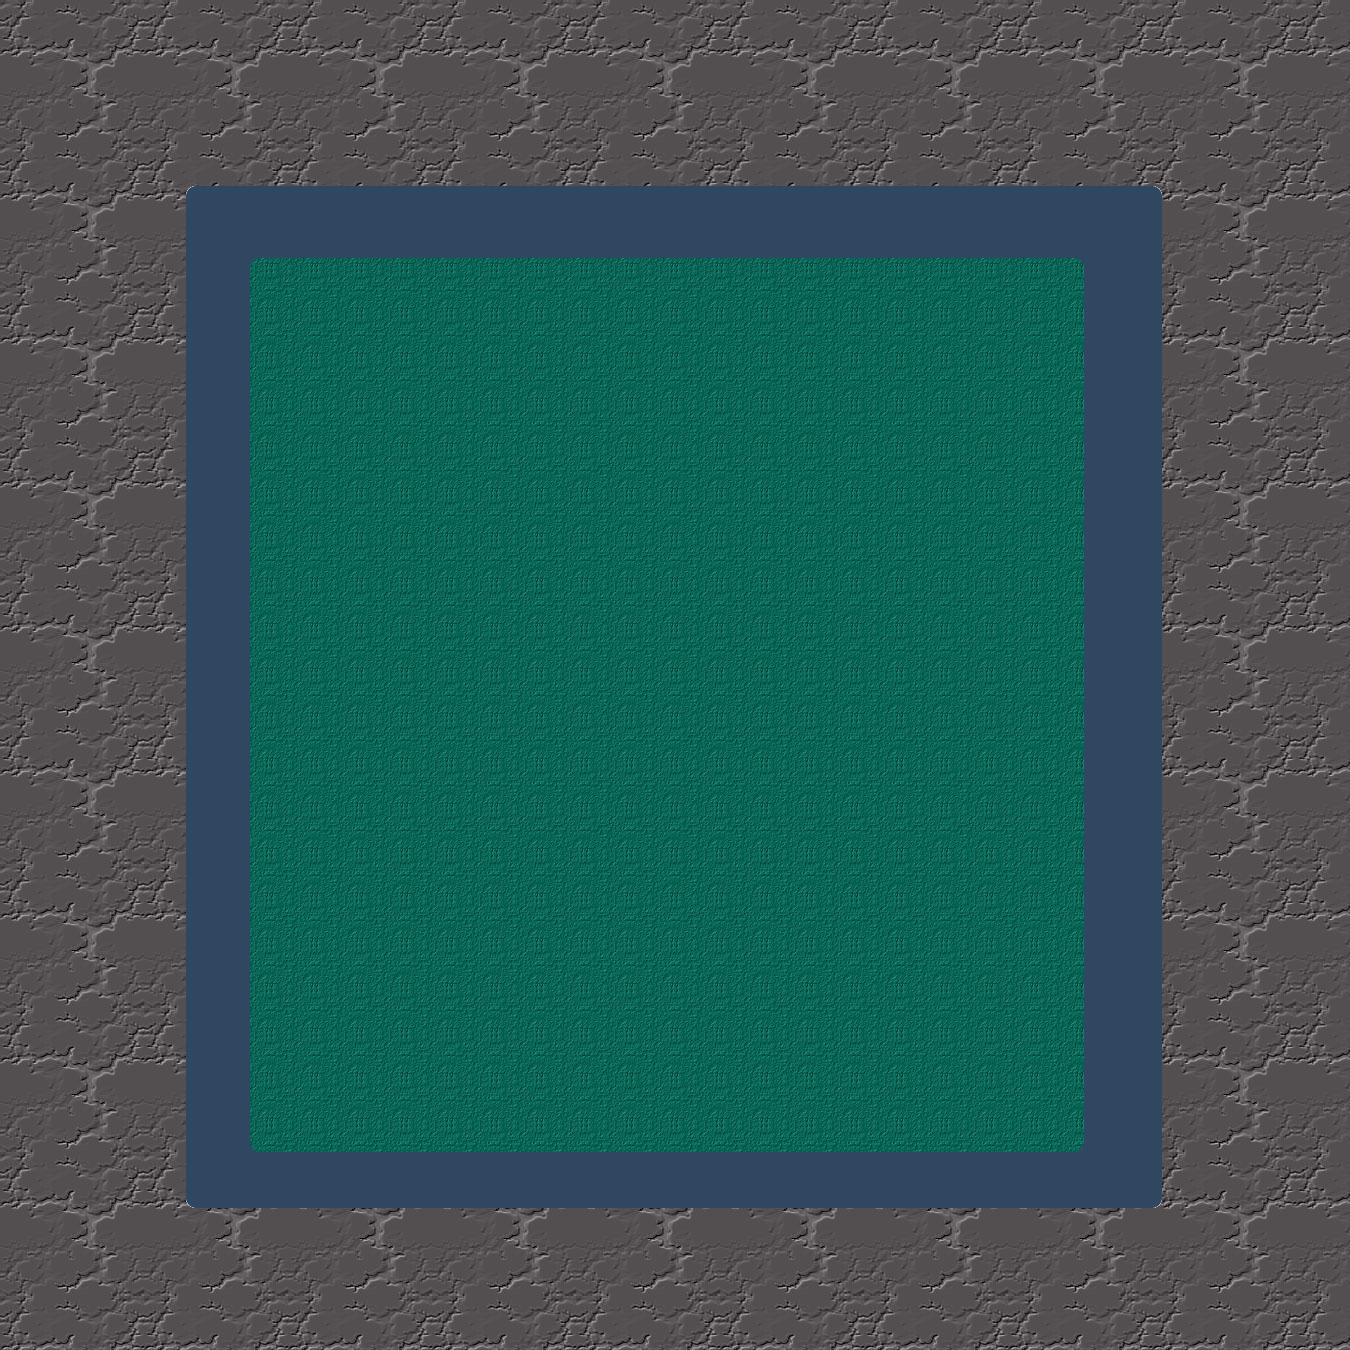
\includegraphics[scale=0.4]{media/Logo.png}\\[5ex]

\singlespacing

\Large{\textbf{\textsc{\art}}}\\[1.5ex]

\singlespacing

\large{\textbf{\textsc{\titlename}}}\\[3ex]

% \LARGE{\textbf{\subtitlename}}\\[4ex]
% \Large{im Studiengang \studienbereich}\\[6ex]

\singlespacing

\large{
    \authornameemailto\\[1.0ex]
    \authoraddress\\[1.0ex]
    \authorlocation\\[1.0ex]
}

\singlespacing

\normalsize
\begin{tabular}{z{5.4cm}p{6cm}}\\
 Matrikelnummer:    & \quad \matrikelnr\\[1.2ex]
 Studiengang:       & \quad \studiengang\\[1.2ex]
 Erstgutachter:     & \quad \erstgutachter\\[1.2ex]
 Zweitgutachter:    & \quad \zweitgutachter\\[1.2ex]
 Ausgabedatum:      & \quad \ausgabedatum\\[1.2ex]
\end{tabular}

\singlespacing

\singlespacing

vorgelegt am \abgabedatum \space zur Erlangung des akademischen Grades\\[1.2ex]
\akademischergrad\\[1.2ex]

\end{center}

\end{titlepage}

\newpage
\cleardoublepage

% ____ Affidavit-Page ______________________________________
%%%%%%%%%%%%%%%%%%%%%%%%%%%%%%%%%%%%%%%%%%%%%%%%%%%%%%%%%%%%
%%%%%%%%%%%              Affidavit               %%%%%%%%%%%
%%%%%%%%%%%%%%%%%%%%%%%%%%%%%%%%%%%%%%%%%%%%%%%%%%%%%%%%%%%%
%
% ____ Affidavit ___________________________________________
%
\chapter*{Affidavit}
\thispagestyle{empty}

I certify that I have written this thesis independently without outside help and that I have used only the sources indicated.

\vspace{3cm}

\begin{tabular}{p{7cm}p{.5cm}l}
\hrulefill  \\
%\dotfill \\
\centering Place, Date
\end{tabular}% 
\hfill
\begin{tabular}{p{7cm}p{.5cm}l}
\hrulefill \\
%\dotfill \\
\centering Signature
%\centering\authorname
\end{tabular}% 

\cleardoublepage

% ____ User-Informations ___________________________________
\pagenumbering{roman}
\setcounter{page}{1}

% ____ Preword _____________________________________________
\chapter*{Vorwort}
%\addcontentsline{toc}{chapter}{Vorwort}
\thispagestyle{empty}

\begin{displayquote}
\textit{Niemand meint alles was er sagt.}
\end{displayquote}

\textbf{Was ist Merkmalsextraktion?}
Merkmalsextraktion ist ein Prozess der Dimensionalitätsreduktion, bei dem ein anfänglicher Satz von Rohdaten zur Verarbeitung auf besser handhabbare Gruppen reduziert wird. Ein Merkmal dieser großen Datensätze ist eine große Anzahl von Variablen, deren Verarbeitung eine Menge an Rechenressourcen erfordert. Merkmalsextraktion ist die Bezeichnung für Methoden, die Variablen auswählen und/oder zu Merkmalen kombinieren, wodurch die Menge der zu verarbeitenden Daten effektiv reduziert wird, während der ursprüngliche Datensatz immer noch genau und vollständig beschrieben wird.

\noindent
\textbf{Warum ist dies nützlich?}

Der Prozess der Merkmalsextraktion ist nützlich, wenn Sie die Anzahl der für die Verarbeitung benötigten Ressourcen reduzieren müssen, ohne wichtige oder relevante Informationen zu verlieren. Die Merkmalsextraktion kann auch die Menge der redundanten Daten für eine bestimmte Analyse reduzieren. Außerdem erleichtern die Reduzierung der Daten und die Bemühungen des Rechners, variable Kombinationen (Merkmale) zu bilden, die Geschwindigkeit der Lern- und Generalisierungsschritte im maschinellen Lernprozess.

\textbf{Praktische Anwendungen der Merkmalsextraktion}

\textbf{Autoencoder}
- Der Zweck von Autoencodierern ist das unbeaufsichtigte Erlernen einer effizienten Datencodierung. Die Merkmalsextraktion wird hier verwendet, um Schlüsselmerkmale in den zu kodierenden Daten zu identifizieren, indem aus der Kodierung des ursprünglichen Datensatzes gelernt wird, um neue Merkmale abzuleiten.

\textbf{Worttasche}
- Eine Technik zur Verarbeitung natürlicher Sprache, die die in einem Satz, Dokument, einer Website usw. verwendeten Wörter (Merkmale) extrahiert und nach der Häufigkeit ihrer Verwendung klassifiziert. Diese Technik kann auch in der Bildverarbeitung angewendet werden.

Im Anschluss dieser Bachelorarbeit wird ein Fazit aus den Erkenntnissen gezogen.


\cleardoublepage

% ____ Abstract ____________________________________________
%%%%%%%%%%%%%%%%%%%%%%%%%%%%%%%%%%%%%%%%%%%%%%%%%%%%%%%%%%%%
%%%%%%%%%%%               Abstract               %%%%%%%%%%%
%%%%%%%%%%%%%%%%%%%%%%%%%%%%%%%%%%%%%%%%%%%%%%%%%%%%%%%%%%%%
%
% ____ Abstract ____________________________________________
%
\chapter*{Abstract}
%\addcontentsline{toc}{chapter}{Abstract}
\thispagestyle{empty}

\lipsum[1]

\vspace{0.5cm}

\textbf{Keywords}:  \keywords

\cleardoublepage

% ____ Acknowledgement _____________________________________
\chapter*{Dankesagung}
%\addcontentsline{toc}{chapter}{Dankesagung}
\thispagestyle{empty}
%\thispagestyle{plain}

\begin{displayquote}
\textit{Niemand meint alles was er sagt, und nur wenige sagen alles was sie denken. Worte sind glitschig und Gedanken sind klebrig. - Henry Adams}
\end{displayquote}

\begin{displayquote}
\textit{Viele Missverständnisse entstehen dadurch, dass ein Dank nicht ausgesprochen, sondern nur empfunden wird. - Ernst R. Hauschka}
\end{displayquote}
Hier kommt mein besonderer Dank hinein, wenn ich dann wirklich einen Aussprechen kann.


\newpage
\cleardoublepage

% ____ Table of Contents ___________________________________
%%%%%%%%%%%%%%%%%%%%%%%%%%%%%%%%%%%%%%%%%%%%%%%%%%%%%%%%%%%%
%%%%%%%%%%%           Table of Contents          %%%%%%%%%%%
%%%%%%%%%%%%%%%%%%%%%%%%%%%%%%%%%%%%%%%%%%%%%%%%%%%%%%%%%%%%

\setcounter{secnumdepth}{4}         % Tiefe der Nummerierung der Kapitel
\setcounter{tocdepth}{3}            % Tiefe des Inhaltsverzeichnis

\makeatletter
\renewcommand*\l@section{\@dottedtocline{1}{1.5em}{2.3em}}
\renewcommand*\l@subsection{\@dottedtocline{2}{3.8em}{3.2em}}
\renewcommand*\l@subsubsection{\@dottedtocline{3}{7.0em}{4.1em}}
\renewcommand*\l@paragraph{\@dottedtocline{4}{10em}{5em}}
\renewcommand*\l@subparagraph{\@dottedtocline{5}{12em}{6em}}
\makeatother

%\RedeclareSectionCommand[style=section, beforeskip=-3.5ex plus -1ex minus -.2ex, afterskip=2.3ex plus.2ex,
%   font=\normalfont\LARGE\bfseries, indent=0pt, tocindent=0em, tocnumwidth=1.5em]{part}
 
%\RedeclareSectionCommand[tocindent=1em, tocnumwidth=1em]{chapter}
%\RedeclareSectionCommand[tocindent=1em, tocnumwidth=2em]{section}
%\RedeclareSectionCommand[tocindent=2em, tocnumwidth=1.5em]{subsection}
%\RedeclareSectionCommand[tocindent=3em, tocnumwidth=1.5em]{subsubsection}
 
%\DeclareSectionCommand[level=4,style=section,
%   beforeskip=-3.25ex plus -1ex minus -.2ex, afterskip=1.5ex plus .2ex,
%   font=\normalfont\normalsize\bfseries, counterwithin=subsubsection,
%   indent=0pt,tocindent=4em, tocnumwidth=1.5em]{subsubsubsection}




%\thispagestyle{empty}                                  % disable numbering
\addtocontents{toc}{\protect\thispagestyle{empty}}      % more then 1 page
\renewcommand*{\tableofcontents}{\listoftoc[{\contentsname}]{toc}}% ToC under control of tocbasic
\AfterTOCHead[toc]{\thispagestyle{empty}\pagestyle{empty}}
\AfterStartingTOC[toc]{\clearpage}
%
\cleardoublepage
%
%\addcontentsline{toc}{chapter}{Inhaltsverzeichnis}     % Inhaltsverzeichnis zum Inhaltsverzeichnis hinzufügen
\renewcommand{\contentsname}{Inhaltsverzeichnis}
\tableofcontents % Inhaltsverzeichnis
% ----------------------------------------------------------

% ____ List of Figures _____________________________________
\renewcommand{\listfigurename}{Abbildungsverzeichnis}
\listoffigures % Abbildungsverzeichnis
\pagenumbering{roman}

% ____ List of Tables ______________________________________
% \setcounter{table}{0} \renewcommand{\thetable}{\arabic{table}}        % change numbering-format
\renewcommand{\listtablename}{Tabellenverzeichnis}
\listoftables % Tabellenverzeichnis

% ____ Acronym _____________________________________________
\printglossary[title=Abkürzungsverzeichnis, nogroupskip, nonumberlist, type=\acronymtype, style=superheader]
%\printglossary[title=Abkürzungsverzeichnis, nogroupskip, nonumberlist, type=\acronymtype, style=super]

% ____ Symbols _____________________________________________
% \printglossary[type=symbolslist, style=long]

% ____ Glossar _____________________________________________
%\printglossary[title=Glossar, nonumberlist, style=tree]
%\newpage\null\thispagestyle{empty}\newpage                  % Empty Page

% ____ List of Listings ____________________________________
%\renewcommand{\lstlistlistingname}{Verzeichnis der Listings}
%\lstlistoflistings  % Listings-Verzeichnis
% ----------------------------------------------------------

% ...danach in normalen arabischen Ziffern -----------------
\cleardoublepage
\pagenumbering{arabic}
\setcounter{page}{1}

% ____ Content _____________________________________
\chapterimage{media/ChapterImage.png}
\chapter{Einführung}
\label{cha:einfuehrung}

\epigraph{Many of life's failures are people who did not realize\\how close they were to success when they gave up.}{Thomas A. Edison}

\section{Einleitung}
\label{sec:einleitung}

How to cite \cite{yt:online}.

\lipsum[9]

\section{Motivation}
\label{sec:motivation}

\begin{figure}[!ht]
    \centering
    
\includegraphics[width=0.9\linewidth]{media/placeholder.png}
    \caption[Platzhalter]{Platzhalter}
    \label{fig:srs_process}
\end{figure}

\lipsum[9]

\section{Ziel der Arbeit}
\label{sec:zielderarbeit}

\lipsum[1]

%\begin{enumerate}[label=\textbf{S.\arabic*},ref=S.\arabic*]
\begin{enumerate}[label=\textit{\textbf{Forschungsfrage \#\arabic*}}, leftmargin=4.25cm, resume]
    \item \label{FF1} \glqq ?\grqq{}
    \item \label{FF2} \glqq ?\grqq{}
    \item \label{FF3} \glqq ?\grqq{}
\end{enumerate}

\lipsum[1]

\section{Abgrenzungen}
\label{sec:abgrenzungen}

\lipsum[2]

\section{Vergleichende Arbeiten}
\label{cha:relatedwork}

\lipsum[2]

\clearpage

\textbf{\autoref{cha:grundlagennlp}: \nameref{cha:grundlagennlp}}\\
\lipsum[2]

\textbf{\autoref{cha:durchfuehrungfeature}: \nameref{cha:durchfuehrungfeature}}\\
\lipsum[2]

\textbf{\autoref{cha:implementierung}: \nameref{cha:implementierung}}\\
\lipsum[2]

\textbf{\autoref{cha:ergebnisse}: \nameref{cha:ergebnisse}}\\
\lipsum[2]

\textbf{\autoref{cha:fazit}: \nameref{cha:fazit}}\\
\lipsum[2]

\setcounter{table}{0} \renewcommand{\thetable}{\arabic{table}}
\chapterimage{media/ChapterImage.png}
\chapter{Grundlagen natürlicher Sprachverarbeitung}
\label{cha:grundlagennlp}

\epigraph{\glqq I think you might be hiring data scientists\\the way a drug lord buys a tiger for his backyard\grqq{}, I told him.\\ \glqq You don’t know what you want with the tiger, but all the other drug lords have one.\grqq{}}{Cassie Kozyrkov, Chief Decision Scientist at Google}

\section{Allgemeines}
\label{sec:allgemeines}

\lipsum[3]

\begin{figure}[!ht]
    \centering
    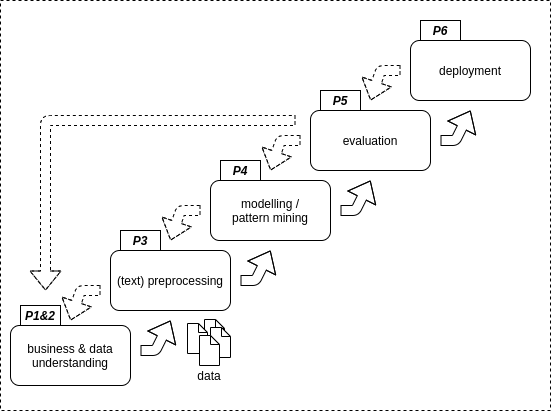
\includegraphics[width=0.9\linewidth]{media/nlp-workflow.png}
    \caption{CRISP-DM 1.0 Modell (eigene, abgeänderte Darstellung)}
    \label{fig:nlp_workflow}
\end{figure}

\lipsum[1]

\subsection{Maschinelles Lernen}
\label{sec:maschinelleslernen}

\lipsum[2]

\subsection{SpaCy Architektur}
\label{sec:spacyarchitektur}

\lipsum[1]

\section{Text Vorverarbeitung}
\label{subsec:textvorverarbeitung}

\lipsum[3]

\subsection{Tokenisierung}
\label{subsec:tokenisierung}

\lipsum[3]

\subsection{Stoppwörter entfernen}
\label{subsec:stoppwörter}

\lipsum[3]

\subsection{Wortart / Part of Speech}
\label{subsec:pos}

\lipsum[3]

\begin{figure}[!ht]
    \centering
    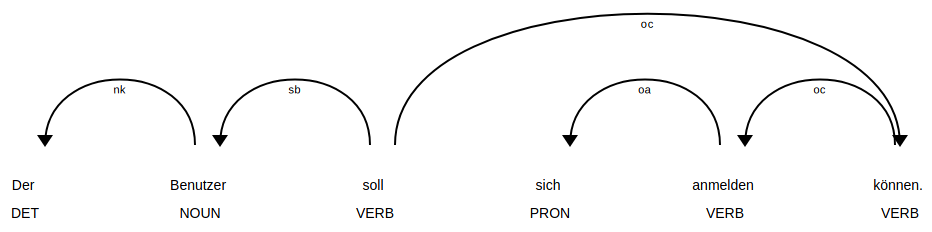
\includegraphics[width=\linewidth]{media/displaCy.png}
    \caption{POS-Muster und Abhängigkeit der Wörter}
    \label{fig:spacy_dependency}
\end{figure}

\lipsum[3]

\subsection{Lemmatisierung}
\label{subsec:lemmatisierung}

\lipsum[3]

\section{Merkmalextraktion}
\label{sec:merkmalextraktion}

\lipsum[3]

\section{Themenmodellierung mit LDA}
\label{subsec:themenmodellierung}

\lipsum[3]

\begin{figure}[!ht]
    \centering
    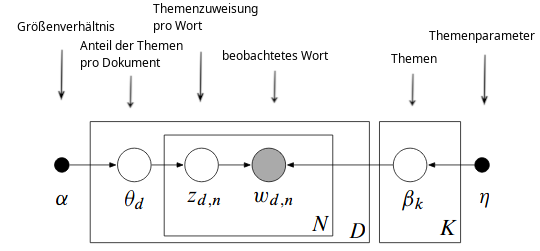
\includegraphics[width=0.9\linewidth]{media/LDA_selbst.png}
    \caption[LDA als grafisches Model mit eigenen Beschriftungen]{LDA als grafisches Modell}
    \label{fig:lda}
\end{figure}

\lipsum[3]

\section{Evaluierung}
\label{sec:evaluierng}

\lipsum[3]

\subsection{Konfusionsmatrix}
\label{sec:konfusionsmatrix}

\lipsum[3]

\begin{table}[!ht]
    \centering
    \begin{adjustbox}{width=0.65\columnwidth, center}
    \resizebox{\textwidth}{!}{
        \begin{tabular}{cccc}
         &  & \multicolumn{2}{c}{\textit{Vorhergesagt}} \\ \cline{3-4} 
         & \multicolumn{1}{c|}{} & \multicolumn{1}{c|}{Positiv} & \multicolumn{1}{c|}{Negativ} \\ \cline{2-4} 
        \multicolumn{1}{c|}{\multirow{2}{*}{\textit{Tatsächlich}}} & \multicolumn{1}{c|}{True} & \multicolumn{1}{c|}{TP} & \multicolumn{1}{c|}{FN} \\ \cline{2-4} 
        \multicolumn{1}{c|}{} & \multicolumn{1}{c|}{False} & \multicolumn{1}{c|}{FP} & \multicolumn{1}{c|}{TN} \\ \cline{2-4}
        \end{tabular}
    }
    \end{adjustbox}
    \caption{Konfusionsmatrix}
    \label{tab:confusionmatrix}
\end{table}

\lipsum[3]

\begin{eqnarray}
    F1 = 2\cdot \frac{precision\cdot recall}{precision+ recall}
\end{eqnarray}

\input{content/03_Durchführung_Features}
\input{content/04_Durchführung_Integration}
\chapterimage{media/ChapterImage.png}
\chapter{Evaluierung und Diskussion der Ergebnisse}
\label{cha:ergebnisse}

\epigraph{No one learns as much about a subject as one who is forced to teach it.}{Peter F. Drucker}

\section{\autoref{cha:durchfuehrungfeature}: \nameref{cha:durchfuehrungfeature}}

\lipsum[3]

\newcommand{\specialcell}[2][c]{%
\begin{tabular}[#1]{@{}c@{}}#2\end{tabular}}

%%%%%%%%%%%%%
%%%% PH_KTC01
\begin{table}[!ht]
    \begin{subtable}{0.465\textwidth}
    \centering
        \resizebox{0.60\textwidth}{!}{%
        \begin{tabular}{cc|cc}
            \multicolumn{1}{c}{} &\multicolumn{1}{c}{} &\multicolumn{2}{c}{\scriptsize Vorhergesagt} \\ 
            \multicolumn{1}{c}{} & 
            \multicolumn{1}{c|}{} & 
            \multicolumn{1}{c}{Wahr} & 
            \multicolumn{1}{c}{Falsch} \\ \hline
            \multirow[c]{2}{*}{\rotatebox[origin=tr]{90}{\tiny Tatsächlich}}
            & Wahr      & 85     & 46     \\ [1.5ex]
            & Falsch    & 114    & 58    \\ \hline
        \end{tabular}
        }
        \caption{SAFE Confusion Matrix}
        \label{cmKTC01safe}
    \end{subtable}
    \hspace{0.2cm}
    \begin{subtable}{0.465\textwidth}
    \centering
        \resizebox{0.60\textwidth}{!}{%
        \begin{tabular}{cc|cc}
            \multicolumn{1}{c}{} &\multicolumn{1}{c}{} &\multicolumn{2}{c}{\scriptsize Vorhergesagt} \\ 
            \multicolumn{1}{c}{} & 
            \multicolumn{1}{c|}{} & 
            \multicolumn{1}{c}{Wahr} & 
            \multicolumn{1}{c}{Falsch} \\ \hline
            \multirow[c]{2}{*}{\rotatebox[origin=tr]{90}{\tiny Tatsächlich}}
            & Wahr      & 77    & 54     \\ [1.5ex]
            & Falsch    & 60    & 112    \\ \hline
        \end{tabular}
        }
        \caption{thesis Confusion Matrix}
        \label{cmKTC01thesis}
    \end{subtable}
    \vspace{0.1cm}
    \begin{subtable}{0.465\textwidth}
    \centering
        \resizebox{\textwidth}{!}{%
        \begin{tabular}{
        >{\columncolor[HTML]{FFFFFF}}r 
        >{\columncolor[HTML]{FFFFFF}}r 
        >{\columncolor[HTML]{FFFFFF}}r 
        >{\columncolor[HTML]{FFFFFF}}r 
        >{\columncolor[HTML]{FFFFFF}}r }
        \multicolumn{1}{l}{\cellcolor[HTML]{FFFFFF}} &
          \multicolumn{1}{l}{\cellcolor[HTML]{FFFFFF}precision} &
          \multicolumn{1}{l}{\cellcolor[HTML]{FFFFFF}recall} &
          \multicolumn{1}{l}{\cellcolor[HTML]{FFFFFF}f1-score} &
          \multicolumn{1}{l}{\cellcolor[HTML]{FFFFFF}support} \\ \cline{2-5} 
        \multicolumn{1}{r|}{\cellcolor[HTML]{FFFFFF}}             &      &      &      & \multicolumn{1}{r|}{\cellcolor[HTML]{FFFFFF}}    \\ \cline{1-1}
        \multicolumn{1}{|r}{\cellcolor[HTML]{FFFFFF}0}            & 0.55 & 0.34 & 0.42 & \multicolumn{1}{r|}{\cellcolor[HTML]{FFFFFF}171}  \\ \hline
        \multicolumn{1}{|r}{\cellcolor[HTML]{FFFFFF}1}            & 0.43 & 0.65 & 0.52 & \multicolumn{1}{r|}{\cellcolor[HTML]{FFFFFF}132}  \\ \hline
                                                                  &      &      &      &                                                  \\ \hline
        \multicolumn{1}{|r}{\cellcolor[HTML]{FFFFFF}accuray}      &      &      & 0.47 & \multicolumn{1}{r|}{\cellcolor[HTML]{FFFFFF}303} \\
        \multicolumn{1}{|r}{\cellcolor[HTML]{FFFFFF}macro avg}    & 0.33 & 0.33 & 0.31 & \multicolumn{1}{r|}{\cellcolor[HTML]{FFFFFF}303} \\
        \multicolumn{1}{|r}{\cellcolor[HTML]{FFFFFF}weighted avg} & 0.50 & 0.47 & 0.46 & \multicolumn{1}{r|}{\cellcolor[HTML]{FFFFFF}303} \\ \hline
        \end{tabular}%
        }
        \caption{SAFE POS-Muster}
        \label{csKTC01safe}
    \end{subtable}
    \hspace{0.2cm}
    \begin{subtable}{0.465\textwidth}
    \centering
        \resizebox{\textwidth}{!}{%
        \begin{tabular}{
        >{\columncolor[HTML]{FFFFFF}}r 
        >{\columncolor[HTML]{FFFFFF}}r 
        >{\columncolor[HTML]{FFFFFF}}r 
        >{\columncolor[HTML]{FFFFFF}}r 
        >{\columncolor[HTML]{FFFFFF}}r }
        \multicolumn{1}{l}{\cellcolor[HTML]{FFFFFF}} &
          \multicolumn{1}{l}{\cellcolor[HTML]{FFFFFF}precision} &
          \multicolumn{1}{l}{\cellcolor[HTML]{FFFFFF}recall} &
          \multicolumn{1}{l}{\cellcolor[HTML]{FFFFFF}f1-score} &
          \multicolumn{1}{l}{\cellcolor[HTML]{FFFFFF}support} \\ \cline{2-5} 
        \multicolumn{1}{r|}{\cellcolor[HTML]{FFFFFF}}             &      &      &      & \multicolumn{1}{r|}{\cellcolor[HTML]{FFFFFF}}    \\ \cline{1-1}
        \multicolumn{1}{|r}{\cellcolor[HTML]{FFFFFF}0}            & 0.67 & 0.65 & 0.66 & \multicolumn{1}{r|}{\cellcolor[HTML]{FFFFFF}171}  \\ \hline
        \multicolumn{1}{|r}{\cellcolor[HTML]{FFFFFF}1}            & 0.57 & 0.59 & 0.58 & \multicolumn{1}{r|}{\cellcolor[HTML]{FFFFFF}132}  \\ \hline
                                                                  &      &      &      &                                                  \\ \hline
        \multicolumn{1}{|r}{\cellcolor[HTML]{FFFFFF}accuray}      &      &      & 0.62 & \multicolumn{1}{r|}{\cellcolor[HTML]{FFFFFF}303} \\
        \multicolumn{1}{|r}{\cellcolor[HTML]{FFFFFF}macro avg}    & 0.41 & 0.41 & 0.41 & \multicolumn{1}{r|}{\cellcolor[HTML]{FFFFFF}303} \\
        \multicolumn{1}{|r}{\cellcolor[HTML]{FFFFFF}weighted avg} & 0.62 & 0.62 & 0.62 & \multicolumn{1}{r|}{\cellcolor[HTML]{FFFFFF}303} \\ \hline
        \end{tabular}%
        }
        \caption{thesis POS-Muster}
        \label{csKTC01thesis}
    \end{subtable}%
    \caption{Konfusionsmatrizen und Kennzahlen des PH\_KTC01}
    \label{tabs:resultsPHKTC01}
\end{table}

\lipsum[3]

\begin{figure}
     \centering
     \begin{subfigure}[b]{0.495\textwidth}
         \centering
         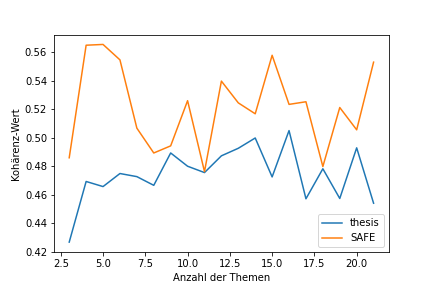
\includegraphics[width=\textwidth]{media/cs_PH_KTC01.png}
         \caption{PH\_KTC01}
         \label{fig:lda-ktc01}
     \end{subfigure}
     \hfill
     \begin{subfigure}[b]{0.495\textwidth}
         \centering
         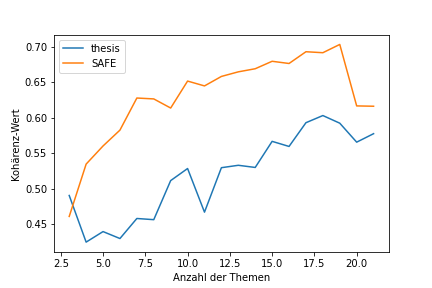
\includegraphics[width=\textwidth]{media/cs_PH_KTC02.png}
         \caption{PH\_KTC02}
         \label{fig:lda-ktc02}
     \end{subfigure}
    \caption{Ergebnisse der Themenmodellierung: PH\_KTC01-02}
    \label{figs:tmtopiccoherence}
\end{figure}

\lipsum[1]

\section{Diskussion}
\label{sec:diskussion}

\lipsum[3]

\chapterimage{media/headerLogo.png}
\chapter{Fazit und Ausblick}
\label{cha:fazit}

\epigraph{Lernen ist Erfahrung. Alles andere ist einfach nur Information.}{Albert Einstein, Physiker}

\section{Zusammenfassung}
\label{sec:zusammenfassung}

\lipsum[4]

\section{Ausblick}
\label{sec:ausblick}

\lipsum[4]

\cleardoublepage
\newpage
\pagenumbering{Roman}

% ____ Bibliography ________________________________
%		Link: http://de.wikipedia.org/wiki/Bib-TeX
%
\printbibliography[title=Literaturverzeichnis, heading=bibintoc]
%\printbibliography[type=article,title={Articles only}]
%\printbibliography[type=book,title={Books only}]
%\printbibliography[keyword={physics},title={Physics-related only}]
%\printbibliography[keyword={latex},title={\LaTeX-related only}]
% --------------------------------------------------

% ____ Appendix ____________________________________
\begin{appendix}
%\setcounter{page}{5}
%%%%%%%%%%%%%%%%%%%%%%%%%%%%%%%%%%%%%%%%%%%%%%%%%%%%%%%%%%%%
%%%%%%%%%%%               Appendix               %%%%%%%%%%%
%%%%%%%%%%%%%%%%%%%%%%%%%%%%%%%%%%%%%%%%%%%%%%%%%%%%%%%%%%%%
%
% ____ Appendix ____________________________________________
%
\chapter{Appendix}
\label{appendix}

\chapterimage{media/ChapterImage.png}
\section{Software used}
\label{sec:software-used}

\vspace{3cm}

\begin{savenotes}
    \begin{table}[!ht]
    \centering
        \begin{tabular}{lll}
        \rowcolor[HTML]{FFFFFF} 
        \textbf{Software} & \textbf{Kategorie} & \textbf{Version} \\ \hline
        \rowcolor[HTML]{FFFFFF} 
        Python & Programmiersprache & 3.8.3\\
        \rowcolor[HTML]{EFEFEF} 
        pdfminer.six\footnote{Webseite: \url{https://pypi.org/project/pdfminer.six/}} & Informationsextraktion & 20200517\\
        \rowcolor[HTML]{FFFFFF}
        pyLDAviz\footnote{Github: \url{https://github.com/bmabey/pyLDAvis}} & Themenmodellierung & 2.1.2\\
        \rowcolor[HTML]{EFEFEF} 
        Gensim\footnote{Webseite: \url{https://radimrehurek.com/gensim}} & Themenmodellierung & 3.8.3\\
        \rowcolor[HTML]{FFFFFF} 
        spaCy\footnote{Github: \url{https://github.com/explosion/spaCy}} & NLP & 2.2.4\\
        \rowcolor[HTML]{EFEFEF} 
        scikit-learn\footnote{Webseite: \url{https://scikit-learn.org}} & Maschinelles Lernen & 0.23.1\\
        Jupyter Lab\footnote{Webseite: \url{https://jupyter.org}} & IDE & 2.1.4\\
        \rowcolor[HTML]{EFEFEF} 
        pandas\footnote{Webseite: \url{https://pandas.pydata.org}} & Datenverwaltung & 1.0.4\\
        \rowcolor[HTML]{FFFFFF} 
        NumPy\footnote{Webseite: \url{https://numpy.org}} & wissenschaftliches Rechnen & 1.18.4\\

        \end{tabular}%
    \caption{Übersicht der verwendeten Software}
    \label{tab:used-software}
    \end{table}
\end{savenotes}

\clearpage

\section{Konfusionsmatrizen der externen Pflichtenhefte}
\label{app:pflichtenhefte}

\vspace{2cm}

%%%%%%%%%%%
%%%% PH_A01
\begin{table}[!ht]
    \begin{subtable}{0.465\textwidth}
    \centering
        \resizebox{0.60\textwidth}{!}{%
        \begin{tabular}{cc|cc}
            \multicolumn{1}{c}{} &\multicolumn{1}{c}{} &\multicolumn{2}{c}{\scriptsize Vorhergesagt} \\ 
            \multicolumn{1}{c}{} & 
            \multicolumn{1}{c|}{} & 
            \multicolumn{1}{c}{Wahr} & 
            \multicolumn{1}{c}{Falsch} \\ \hline
            \multirow[c]{2}{*}{\rotatebox[origin=tr]{90}{\tiny Tatsächlich}}
            & Wahr      & 109    & 65     \\ [1.5ex]
            & Falsch    & 36    & 24    \\ \hline
        \end{tabular}
        }
        \caption{SAFE Confusion Matrix}
        \label{cmA01safe}
    \end{subtable}
    \hspace{0.2cm}
    \begin{subtable}{0.465\textwidth}
    \centering
        \resizebox{0.60\textwidth}{!}{%
        \begin{tabular}{cc|cc}
            \multicolumn{1}{c}{} &\multicolumn{1}{c}{} &\multicolumn{2}{c}{\scriptsize Vorhergesagt} \\ 
            \multicolumn{1}{c}{} & 
            \multicolumn{1}{c|}{} & 
            \multicolumn{1}{c}{Wahr} & 
            \multicolumn{1}{c}{Falsch} \\ \hline
            \multirow[c]{2}{*}{\rotatebox[origin=tr]{90}{\tiny Tatsächlich}}
            & Wahr      & 118   & 56     \\ [1.5ex]
            & Falsch    & 22    & 38    \\ \hline
        \end{tabular}
        }
        \caption{thesis Confusion Matrix}
        \label{cmA01thesis}
    \end{subtable}
    \vspace{0.1cm}
    \begin{subtable}{0.465\textwidth}
    \centering
        \resizebox{\textwidth}{!}{%
        \begin{tabular}{
        >{\columncolor[HTML]{FFFFFF}}r 
        >{\columncolor[HTML]{FFFFFF}}r 
        >{\columncolor[HTML]{FFFFFF}}r 
        >{\columncolor[HTML]{FFFFFF}}r 
        >{\columncolor[HTML]{FFFFFF}}r }
        \multicolumn{1}{l}{\cellcolor[HTML]{FFFFFF}} &
          \multicolumn{1}{l}{\cellcolor[HTML]{FFFFFF}precision} &
          \multicolumn{1}{l}{\cellcolor[HTML]{FFFFFF}recall} &
          \multicolumn{1}{l}{\cellcolor[HTML]{FFFFFF}f1-score} &
          \multicolumn{1}{l}{\cellcolor[HTML]{FFFFFF}support} \\ \cline{2-5} 
        \multicolumn{1}{r|}{\cellcolor[HTML]{FFFFFF}}             &      &      &      & \multicolumn{1}{r|}{\cellcolor[HTML]{FFFFFF}}    \\ \cline{1-1}
        \multicolumn{1}{|r}{\cellcolor[HTML]{FFFFFF}0}            & 0.25 & 0.85 & 0.39 & \multicolumn{1}{r|}{\cellcolor[HTML]{FFFFFF}60}  \\ \hline
        \multicolumn{1}{|r}{\cellcolor[HTML]{FFFFFF}1}            & 0.73 & 0.14 & 0.23 & \multicolumn{1}{r|}{\cellcolor[HTML]{FFFFFF}174}  \\ \hline
                                                                  &      &      &      &                                                  \\ \hline
        \multicolumn{1}{|r}{\cellcolor[HTML]{FFFFFF}accuray}      &      &      & 0.32 & \multicolumn{1}{r|}{\cellcolor[HTML]{FFFFFF}234} \\
        \multicolumn{1}{|r}{\cellcolor[HTML]{FFFFFF}macro avg}    & 0.49 & 0.49 & 0.31 & \multicolumn{1}{r|}{\cellcolor[HTML]{FFFFFF}234} \\
        \multicolumn{1}{|r}{\cellcolor[HTML]{FFFFFF}weighted avg} & 0.61 & 0.32 & 0.27 & \multicolumn{1}{r|}{\cellcolor[HTML]{FFFFFF}234} \\ \hline
        \end{tabular}%
        }
        \caption{SAFE POS-Muster}
        \label{csA01safe}
    \end{subtable}
    \hspace{0.2cm}
    \begin{subtable}{0.465\textwidth}
    \centering
        \resizebox{\textwidth}{!}{%
        \begin{tabular}{
        >{\columncolor[HTML]{FFFFFF}}r 
        >{\columncolor[HTML]{FFFFFF}}r 
        >{\columncolor[HTML]{FFFFFF}}r 
        >{\columncolor[HTML]{FFFFFF}}r 
        >{\columncolor[HTML]{FFFFFF}}r }
        \multicolumn{1}{l}{\cellcolor[HTML]{FFFFFF}} &
          \multicolumn{1}{l}{\cellcolor[HTML]{FFFFFF}precision} &
          \multicolumn{1}{l}{\cellcolor[HTML]{FFFFFF}recall} &
          \multicolumn{1}{l}{\cellcolor[HTML]{FFFFFF}f1-score} &
          \multicolumn{1}{l}{\cellcolor[HTML]{FFFFFF}support} \\ \cline{2-5} 
        \multicolumn{1}{r|}{\cellcolor[HTML]{FFFFFF}}             &      &      &      & \multicolumn{1}{r|}{\cellcolor[HTML]{FFFFFF}}    \\ \cline{1-1}
        \multicolumn{1}{|r}{\cellcolor[HTML]{FFFFFF}0}            & 0.40 & 0.63 & 0.49 & \multicolumn{1}{r|}{\cellcolor[HTML]{FFFFFF}60}  \\ \hline
        \multicolumn{1}{|r}{\cellcolor[HTML]{FFFFFF}1}            & 0.84 & 0.68 & 0.75 & \multicolumn{1}{r|}{\cellcolor[HTML]{FFFFFF}174}  \\ \hline
                                                                  &      &      &      &                                                  \\ \hline
        \multicolumn{1}{|r}{\cellcolor[HTML]{FFFFFF}accuray}      &      &      & 0.67 & \multicolumn{1}{r|}{\cellcolor[HTML]{FFFFFF}234} \\
        \multicolumn{1}{|r}{\cellcolor[HTML]{FFFFFF}macro avg}    & 0.62 & 0.66 & 0.62 & \multicolumn{1}{r|}{\cellcolor[HTML]{FFFFFF}234} \\
        \multicolumn{1}{|r}{\cellcolor[HTML]{FFFFFF}weighted avg} & 0.73 & 0.67 & 0.69 & \multicolumn{1}{r|}{\cellcolor[HTML]{FFFFFF}234} \\ \hline
        \end{tabular}%
        }
        \caption{thesis POS-Muster}
        \label{csA01thesis}
    \end{subtable}%
    \caption{Konfusionsmatrizen und Kennzahlen des PH\_A01}
    \label{tabs:resultsPHA01}
\end{table}

\vspace{2cm}

%%%%%%%%%%%
%%%% PH_A02
\begin{table}[!ht]
    \begin{subtable}{0.465\textwidth}
    \centering
        \resizebox{0.60\textwidth}{!}{%
        \begin{tabular}{cc|cc}
            \multicolumn{1}{c}{} &\multicolumn{1}{c}{} &\multicolumn{2}{c}{\scriptsize Vorhergesagt} \\ 
            \multicolumn{1}{c}{} & 
            \multicolumn{1}{c|}{} & 
            \multicolumn{1}{c}{Wahr} & 
            \multicolumn{1}{c}{Falsch} \\ \hline
            \multirow[c]{2}{*}{\rotatebox[origin=tr]{90}{\tiny Tatsächlich}}
            & Wahr      & 48    & 40    \\ [1.5ex]
            & Falsch    & 37    & 18    \\ \hline
        \end{tabular}
        }
        \caption{SAFE Confusion Matrix}
        \label{cmA02safe}
    \end{subtable}
    \hspace{0.2cm}
    \begin{subtable}{0.465\textwidth}
    \centering
        \resizebox{0.60\textwidth}{!}{%
        \begin{tabular}{cc|cc}
            \multicolumn{1}{c}{} &\multicolumn{1}{c}{} &\multicolumn{2}{c}{\scriptsize Vorhergesagt} \\ 
            \multicolumn{1}{c}{} & 
            \multicolumn{1}{c|}{} & 
            \multicolumn{1}{c}{Wahr} & 
            \multicolumn{1}{c}{Falsch} \\ \hline
            \multirow[c]{2}{*}{\rotatebox[origin=tr]{90}{\tiny Tatsächlich}}
            & Wahr      & 62    & 26    \\ [1.5ex]
            & Falsch    & 23    & 32    \\ \hline
        \end{tabular}
        }
        \caption{thesis Confusion Matrix}
        \label{cmA02thesis}
    \end{subtable}
    \vspace{0.1cm}
    \begin{subtable}{0.465\textwidth}
    \centering
        \resizebox{\textwidth}{!}{%
        \begin{tabular}{
        >{\columncolor[HTML]{FFFFFF}}r 
        >{\columncolor[HTML]{FFFFFF}}r 
        >{\columncolor[HTML]{FFFFFF}}r 
        >{\columncolor[HTML]{FFFFFF}}r 
        >{\columncolor[HTML]{FFFFFF}}r }
        \multicolumn{1}{l}{\cellcolor[HTML]{FFFFFF}} &
          \multicolumn{1}{l}{\cellcolor[HTML]{FFFFFF}precision} &
          \multicolumn{1}{l}{\cellcolor[HTML]{FFFFFF}recall} &
          \multicolumn{1}{l}{\cellcolor[HTML]{FFFFFF}f1-score} &
          \multicolumn{1}{l}{\cellcolor[HTML]{FFFFFF}support} \\ \cline{2-5} 
        \multicolumn{1}{r|}{\cellcolor[HTML]{FFFFFF}}             &      &      &      & \multicolumn{1}{r|}{\cellcolor[HTML]{FFFFFF}}    \\ \cline{1-1}
        \multicolumn{1}{|r}{\cellcolor[HTML]{FFFFFF}0}            & 0.31 & 0.33 & 0.32 & \multicolumn{1}{r|}{\cellcolor[HTML]{FFFFFF}55}  \\ \hline
        \multicolumn{1}{|r}{\cellcolor[HTML]{FFFFFF}1}            & 0.56 & 0.55 & 0.55 & \multicolumn{1}{r|}{\cellcolor[HTML]{FFFFFF}88}  \\ \hline
                                                                  &      &      &      &                                                  \\ \hline
        \multicolumn{1}{|r}{\cellcolor[HTML]{FFFFFF}accuray}      &      &      & 0.46 & \multicolumn{1}{r|}{\cellcolor[HTML]{FFFFFF}144} \\
        \multicolumn{1}{|r}{\cellcolor[HTML]{FFFFFF}macro avg}    & 0.29 & 0.29 & 0.29 & \multicolumn{1}{r|}{\cellcolor[HTML]{FFFFFF}144} \\
        \multicolumn{1}{|r}{\cellcolor[HTML]{FFFFFF}weighted avg} & 0.46 & 0.46 & 0.46 & \multicolumn{1}{r|}{\cellcolor[HTML]{FFFFFF}144} \\ \hline
        \end{tabular}%
        }
        \caption{SAFE POS-Muster}
        \label{csA02safe}
    \end{subtable}%
    \hspace{0.2cm}
    \begin{subtable}{0.465\textwidth}
    \centering
        \resizebox{\textwidth}{!}{%
        \begin{tabular}{
        >{\columncolor[HTML]{FFFFFF}}r 
        >{\columncolor[HTML]{FFFFFF}}r 
        >{\columncolor[HTML]{FFFFFF}}r 
        >{\columncolor[HTML]{FFFFFF}}r 
        >{\columncolor[HTML]{FFFFFF}}r }
        \multicolumn{1}{l}{\cellcolor[HTML]{FFFFFF}} &
          \multicolumn{1}{l}{\cellcolor[HTML]{FFFFFF}precision} &
          \multicolumn{1}{l}{\cellcolor[HTML]{FFFFFF}recall} &
          \multicolumn{1}{l}{\cellcolor[HTML]{FFFFFF}f1-score} &
          \multicolumn{1}{l}{\cellcolor[HTML]{FFFFFF}support} \\ \cline{2-5} 
        \multicolumn{1}{r|}{\cellcolor[HTML]{FFFFFF}}             &      &      &      & \multicolumn{1}{r|}{\cellcolor[HTML]{FFFFFF}}    \\ \cline{1-1}
        \multicolumn{1}{|r}{\cellcolor[HTML]{FFFFFF}0}            & 0.54 & 0.58 & 0.56 & \multicolumn{1}{r|}{\cellcolor[HTML]{FFFFFF}55}  \\ \hline
        \multicolumn{1}{|r}{\cellcolor[HTML]{FFFFFF}1}            & 0.73 & 0.70 & 0.72 & \multicolumn{1}{r|}{\cellcolor[HTML]{FFFFFF}88}  \\ \hline
                                                                  &      &      &      &                                                  \\ \hline
        \multicolumn{1}{|r}{\cellcolor[HTML]{FFFFFF}accuray}      &      &      & 0.65 & \multicolumn{1}{r|}{\cellcolor[HTML]{FFFFFF}144} \\
        \multicolumn{1}{|r}{\cellcolor[HTML]{FFFFFF}macro avg}    & 0.42 & 0.43 & 0.43 & \multicolumn{1}{r|}{\cellcolor[HTML]{FFFFFF}144} \\
        \multicolumn{1}{|r}{\cellcolor[HTML]{FFFFFF}weighted avg} & 0.65 & 0.65 & 0.65 & \multicolumn{1}{r|}{\cellcolor[HTML]{FFFFFF}144} \\ \hline
        \end{tabular}%
        }
        \caption{thesis POS-Muster}
        \label{csA02thesis}
    \end{subtable}
    \caption{Konfusionsmatrizen und Kennzahlen des PH\_A02}
    \label{tabs:resultsPHA02}
\end{table}

%%%%%%%%%%%
%%%% PH_A03
\begin{table}[!ht]
    \begin{subtable}{0.465\textwidth}
    \centering
        \resizebox{0.60\textwidth}{!}{%
        \begin{tabular}{cc|cc}
            \multicolumn{1}{c}{} &\multicolumn{1}{c}{} &\multicolumn{2}{c}{\scriptsize Vorhergesagt} \\ 
            \multicolumn{1}{c}{} & 
            \multicolumn{1}{c|}{} & 
            \multicolumn{1}{c}{Wahr} & 
            \multicolumn{1}{c}{Falsch} \\ \hline
            \multirow[c]{2}{*}{\rotatebox[origin=tr]{90}{\tiny Tatsächlich}}
            & Wahr      & 153    & 102     \\ [1.5ex]
            & Falsch    & 108     & 139    \\ \hline
        \end{tabular}
        }
        \caption{SAFE Confusion Matrix}
        \label{cmA03safe}
    \end{subtable}
    \hspace{0.2cm}
    \begin{subtable}{0.465\textwidth}
    \centering
        \resizebox{0.60\textwidth}{!}{%
        \begin{tabular}{cc|cc}
            \multicolumn{1}{c}{} &\multicolumn{1}{c}{} &\multicolumn{2}{c}{\scriptsize Vorhergesagt} \\ 
            \multicolumn{1}{c}{} & 
            \multicolumn{1}{c|}{} & 
            \multicolumn{1}{c}{Wahr} & 
            \multicolumn{1}{c}{Falsch} \\ \hline
            \multirow[c]{2}{*}{\rotatebox[origin=tr]{90}{\tiny Tatsächlich}}
            & Wahr      & 202   & 53    \\ [1.5ex]
            & Falsch    & 81    & 166    \\ \hline
        \end{tabular}
        }
        \caption{thesis Confusion Matrix}
        \label{cmA03thesis}
    \end{subtable}
    \vspace{0.1cm}
    \begin{subtable}{0.465\textwidth}
    \centering
        \resizebox{\textwidth}{!}{%
        \begin{tabular}{
        >{\columncolor[HTML]{FFFFFF}}r 
        >{\columncolor[HTML]{FFFFFF}}r 
        >{\columncolor[HTML]{FFFFFF}}r 
        >{\columncolor[HTML]{FFFFFF}}r 
        >{\columncolor[HTML]{FFFFFF}}r }
        \multicolumn{1}{l}{\cellcolor[HTML]{FFFFFF}} &
          \multicolumn{1}{l}{\cellcolor[HTML]{FFFFFF}precision} &
          \multicolumn{1}{l}{\cellcolor[HTML]{FFFFFF}recall} &
          \multicolumn{1}{l}{\cellcolor[HTML]{FFFFFF}f1-score} &
          \multicolumn{1}{l}{\cellcolor[HTML]{FFFFFF}support} \\ \cline{2-5} 
        \multicolumn{1}{r|}{\cellcolor[HTML]{FFFFFF}}             &      &      &      & \multicolumn{1}{r|}{\cellcolor[HTML]{FFFFFF}}    \\ \cline{1-1}
        \multicolumn{1}{|r}{\cellcolor[HTML]{FFFFFF}0}            & 0.58 & 0.56 & 0.57 & \multicolumn{1}{r|}{\cellcolor[HTML]{FFFFFF}247}  \\ \hline
        \multicolumn{1}{|r}{\cellcolor[HTML]{FFFFFF}1}            & 0.59 & 0.60 & 0.59 & \multicolumn{1}{r|}{\cellcolor[HTML]{FFFFFF}255}  \\ \hline
                                                                  &      &      &      &                                                  \\ \hline
        \multicolumn{1}{|r}{\cellcolor[HTML]{FFFFFF}accuray}      &      &      & 0.58 & \multicolumn{1}{r|}{\cellcolor[HTML]{FFFFFF}502} \\
        \multicolumn{1}{|r}{\cellcolor[HTML]{FFFFFF}macro avg}    & 0.58 & 0.58 & 0.58 & \multicolumn{1}{r|}{\cellcolor[HTML]{FFFFFF}502} \\
        \multicolumn{1}{|r}{\cellcolor[HTML]{FFFFFF}weighted avg} & 0.58 & 0.58 & 0.58 & \multicolumn{1}{r|}{\cellcolor[HTML]{FFFFFF}502} \\ \hline
        \end{tabular}%
        }
        \caption{SAFE POS-Muster}
        \label{csA03safe}
    \end{subtable}%
    \hspace{0.2cm}
    \begin{subtable}{0.465\textwidth}
    \centering
        \resizebox{\textwidth}{!}{%
        \begin{tabular}{
        >{\columncolor[HTML]{FFFFFF}}r 
        >{\columncolor[HTML]{FFFFFF}}r 
        >{\columncolor[HTML]{FFFFFF}}r 
        >{\columncolor[HTML]{FFFFFF}}r 
        >{\columncolor[HTML]{FFFFFF}}r }
        \multicolumn{1}{l}{\cellcolor[HTML]{FFFFFF}} &
          \multicolumn{1}{l}{\cellcolor[HTML]{FFFFFF}precision} &
          \multicolumn{1}{l}{\cellcolor[HTML]{FFFFFF}recall} &
          \multicolumn{1}{l}{\cellcolor[HTML]{FFFFFF}f1-score} &
          \multicolumn{1}{l}{\cellcolor[HTML]{FFFFFF}support} \\ \cline{2-5} 
        \multicolumn{1}{r|}{\cellcolor[HTML]{FFFFFF}}             &      &      &      & \multicolumn{1}{r|}{\cellcolor[HTML]{FFFFFF}}    \\ \cline{1-1}
        \multicolumn{1}{|r}{\cellcolor[HTML]{FFFFFF}0}            & 0.75 & 0.67 & 0.71 & \multicolumn{1}{r|}{\cellcolor[HTML]{FFFFFF}247}  \\ \hline
        \multicolumn{1}{|r}{\cellcolor[HTML]{FFFFFF}1}            & 0.71 & 0.78 & 0.74 & \multicolumn{1}{r|}{\cellcolor[HTML]{FFFFFF}255}  \\ \hline
                                                                  &      &      &      &                                                  \\ \hline
        \multicolumn{1}{|r}{\cellcolor[HTML]{FFFFFF}accuray}      &      &      & 0.73 & \multicolumn{1}{r|}{\cellcolor[HTML]{FFFFFF}502} \\
        \multicolumn{1}{|r}{\cellcolor[HTML]{FFFFFF}macro avg}    & 0.73 & 0.73 & 0.73 & \multicolumn{1}{r|}{\cellcolor[HTML]{FFFFFF}502} \\
        \multicolumn{1}{|r}{\cellcolor[HTML]{FFFFFF}weighted avg} & 0.73 & 0.73 & 0.73 & \multicolumn{1}{r|}{\cellcolor[HTML]{FFFFFF}502} \\ \hline
        \end{tabular}%
        }
        \caption{thesis POS-Muster}
        \label{csA03thesis}
    \end{subtable}%
    \caption{Konfusionsmatrizen und Kennzahlen des PH\_A03}
    \label{tabs:resultsPHA03}
\end{table}

%%%%%%%%%%%
%%%% PH_A04
\begin{table}[!ht]
    \begin{subtable}{0.465\textwidth}
    \centering
        \resizebox{0.60\textwidth}{!}{%
        \begin{tabular}{cc|cc}
            \multicolumn{1}{c}{} &\multicolumn{1}{c}{} &\multicolumn{2}{c}{\scriptsize Vorhergesagt} \\ 
            \multicolumn{1}{c}{} & 
            \multicolumn{1}{c|}{} & 
            \multicolumn{1}{c}{Wahr} & 
            \multicolumn{1}{c}{Falsch} \\ \hline
            \multirow[c]{2}{*}{\rotatebox[origin=tr]{90}{\tiny Tatsächlich}}
            & Wahr      & 19     & 13     \\ [1.5ex]
            & Falsch    & 33     & 48    \\ \hline
        \end{tabular}
        }
        \caption{SAFE Confusion Matrix}
        \label{cmA04safe}
    \end{subtable}
    \hspace{0.2cm}
    \begin{subtable}{0.465\textwidth}
    \centering
        \resizebox{0.60\textwidth}{!}{%
        \begin{tabular}{cc|cc}
            \multicolumn{1}{c}{} &\multicolumn{1}{c}{} &\multicolumn{2}{c}{\scriptsize Vorhergesagt} \\ 
            \multicolumn{1}{c}{} & 
            \multicolumn{1}{c|}{} & 
            \multicolumn{1}{c}{Wahr} & 
            \multicolumn{1}{c}{Falsch} \\ \hline
            \multirow[c]{2}{*}{\rotatebox[origin=tr]{90}{\tiny Tatsächlich}}
            & Wahr      & 18    & 14     \\ [1.5ex]
            & Falsch    & 12    & 69    \\ \hline
        \end{tabular}
        }
        \caption{thesis Confusion Matrix}
        \label{cmA04thesis}
    \end{subtable}
    \vspace{0.1cm}
    \begin{subtable}{0.465\textwidth}
    \centering
        \resizebox{\textwidth}{!}{%
        \begin{tabular}{
        >{\columncolor[HTML]{FFFFFF}}r 
        >{\columncolor[HTML]{FFFFFF}}r 
        >{\columncolor[HTML]{FFFFFF}}r 
        >{\columncolor[HTML]{FFFFFF}}r 
        >{\columncolor[HTML]{FFFFFF}}r }
        \multicolumn{1}{l}{\cellcolor[HTML]{FFFFFF}} &
          \multicolumn{1}{l}{\cellcolor[HTML]{FFFFFF}precision} &
          \multicolumn{1}{l}{\cellcolor[HTML]{FFFFFF}recall} &
          \multicolumn{1}{l}{\cellcolor[HTML]{FFFFFF}f1-score} &
          \multicolumn{1}{l}{\cellcolor[HTML]{FFFFFF}support} \\ \cline{2-5} 
        \multicolumn{1}{r|}{\cellcolor[HTML]{FFFFFF}}             &      &      &      & \multicolumn{1}{r|}{\cellcolor[HTML]{FFFFFF}}    \\ \cline{1-1}
        \multicolumn{1}{|r}{\cellcolor[HTML]{FFFFFF}0}            & 0.89 & 0.41 & 0.56 & \multicolumn{1}{r|}{\cellcolor[HTML]{FFFFFF}81}  \\ \hline
        \multicolumn{1}{|r}{\cellcolor[HTML]{FFFFFF}1}            & 0.37 & 0.88 & 0.52 & \multicolumn{1}{r|}{\cellcolor[HTML]{FFFFFF}32}  \\ \hline
                                                                  &      &      &      &                                                  \\ \hline
        \multicolumn{1}{|r}{\cellcolor[HTML]{FFFFFF}accuray}      &      &      & 0.54 & \multicolumn{1}{r|}{\cellcolor[HTML]{FFFFFF}113} \\
        \multicolumn{1}{|r}{\cellcolor[HTML]{FFFFFF}macro avg}    & 0.63 & 0.64 & 0.54 & \multicolumn{1}{r|}{\cellcolor[HTML]{FFFFFF}113} \\
        \multicolumn{1}{|r}{\cellcolor[HTML]{FFFFFF}weighted avg} & 0.74 & 0.54 & 0.55 & \multicolumn{1}{r|}{\cellcolor[HTML]{FFFFFF}113} \\ \hline
        \end{tabular}%
        }
        \caption{SAFE POS-Muster}
        \label{csA04safe}
    \end{subtable}%
    \hspace{0.2cm}
    \begin{subtable}{0.465\textwidth}
    \centering
        \resizebox{\textwidth}{!}{%
        \begin{tabular}{
        >{\columncolor[HTML]{FFFFFF}}r 
        >{\columncolor[HTML]{FFFFFF}}r 
        >{\columncolor[HTML]{FFFFFF}}r 
        >{\columncolor[HTML]{FFFFFF}}r 
        >{\columncolor[HTML]{FFFFFF}}r }
        \multicolumn{1}{l}{\cellcolor[HTML]{FFFFFF}} &
          \multicolumn{1}{l}{\cellcolor[HTML]{FFFFFF}precision} &
          \multicolumn{1}{l}{\cellcolor[HTML]{FFFFFF}recall} &
          \multicolumn{1}{l}{\cellcolor[HTML]{FFFFFF}f1-score} &
          \multicolumn{1}{l}{\cellcolor[HTML]{FFFFFF}support} \\ \cline{2-5} 
        \multicolumn{1}{r|}{\cellcolor[HTML]{FFFFFF}}             &      &      &      & \multicolumn{1}{r|}{\cellcolor[HTML]{FFFFFF}}    \\ \cline{1-1}
        \multicolumn{1}{|r}{\cellcolor[HTML]{FFFFFF}0}            & 0.83 & 0.85 & 0.84 & \multicolumn{1}{r|}{\cellcolor[HTML]{FFFFFF}81}  \\ \hline
        \multicolumn{1}{|r}{\cellcolor[HTML]{FFFFFF}1}            & 0.60 & 0.56 & 0.58 & \multicolumn{1}{r|}{\cellcolor[HTML]{FFFFFF}32}  \\ \hline
                                                                  &      &      &      &                                                  \\ \hline
        \multicolumn{1}{|r}{\cellcolor[HTML]{FFFFFF}accuray}      &      &      & 0.77 & \multicolumn{1}{r|}{\cellcolor[HTML]{FFFFFF}113} \\
        \multicolumn{1}{|r}{\cellcolor[HTML]{FFFFFF}macro avg}    & 0.72 & 0.71 & 0.71 & \multicolumn{1}{r|}{\cellcolor[HTML]{FFFFFF}113} \\
        \multicolumn{1}{|r}{\cellcolor[HTML]{FFFFFF}weighted avg} & 0.77 & 0.77 & 0.77 & \multicolumn{1}{r|}{\cellcolor[HTML]{FFFFFF}113} \\ \hline
        \end{tabular}%
        }
        \caption{thesis POS-Muster}
        \label{csA04thesis}
    \end{subtable}
    \caption{Konfusionsmatrizen und Kennzahlen des PH\_A04}
    \label{tabs:resultsPHA04}
\end{table}

\clearpage

\section{Ergebnisse der Themenmodellierung}

\vspace{4cm}

\begin{figure}[!ht]
     \centering
     \begin{subfigure}[b]{0.495\textwidth}
         \centering
         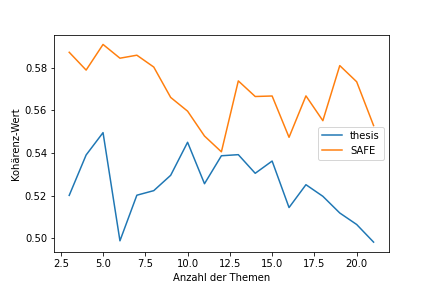
\includegraphics[width=\textwidth]{media/cs_PH_A01.png}
         \caption{PH\_01}
         \label{fig:lda-a01}
     \end{subfigure}
     \hfill
     \begin{subfigure}[b]{0.495\textwidth}
         \centering
         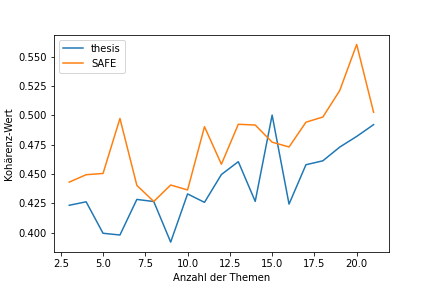
\includegraphics[width=\textwidth]{media/cs_PH_A02.png}
         \caption{PH\_02}
         \label{fig:lda-a02}
     \end{subfigure}
     \hfill
     \begin{subfigure}[b]{0.495\textwidth}
         \centering
         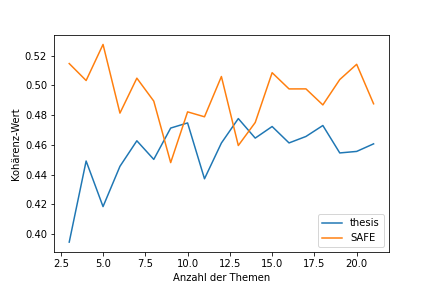
\includegraphics[width=\textwidth]{media/cs_PH_A03.png}
         \caption{PH\_03}
         \label{fig:lda-a03}
     \end{subfigure}
     \hfill
     \begin{subfigure}[b]{0.495\textwidth}
         \centering
         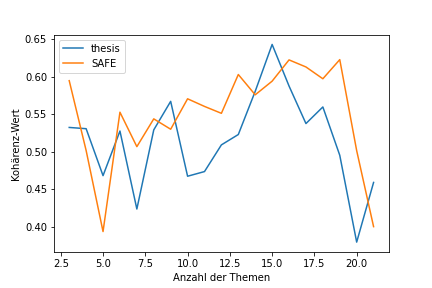
\includegraphics[width=\textwidth]{media/cs_PH_A04.png}
         \caption{PH\_04}
         \label{fig:lda-a04}
     \end{subfigure}
    \caption{Ergebnisse der Themenmodellierung: PH\_A01-04}
    \label{app:figs:tmtopiccoherence-external}
\end{figure}

\section{USB-Massenspeicher}

\vspace{0.5cm}

Auf dem beigelegten USB-Massenspeicher befinden sich:

\begin{itemize}
    \item Bachelorarbeit im PDF-Format
    \item Programmcode
    \begin{itemize}
        \item Jupyter Lab Projekt
        \item PyCharm Projekt
    \end{itemize}
\end{itemize}


\end{appendix}
% --------------------------------------------------

% ____ Index _______________________________________
% \printindex		% Index hier einfügen

% ____ End of Document _____________________________
\end{document}
%
%          .----.__
%         / c  ^  _`;
%         |     .--'
%          \   (
%          /  -.\
%         / .   \
%        /  \    |
%       ;    `-. `.
%       |      /`'.`.
%       |      |   \ \
%       |    __|    `'
%       ;   /   \
%      ,'        |
%     (_`'---._ /--,
%       `'---._`'---..__
%              `''''--, )
%                _.-'`,`
%                 ````
